\documentclass{IEEEoj}

\usepackage{cite}
\usepackage{amsmath,amssymb,amsfonts}
\usepackage{amsthm}
\usepackage{graphicx}
\usepackage{textcomp}
\usepackage{xcolor}
\usepackage{booktabs}
\usepackage{array}
\usepackage{tabularx}
\usepackage{url}
\usepackage{xurl}   % allow long reference URLs to break across lines
\usepackage{multirow}
\usepackage{siunitx}
\usepackage{pgfplots}
\usepackage{tikz}
\usetikzlibrary{shapes.geometric, arrows.meta, positioning, calc, patterns}
\definecolor{lowc}{RGB}{216,90,48}   % low-band, wide-beam links (Fig. 1)
\definecolor{highc}{RGB}{83,74,183}  % high-band, narrow-beam links (Fig. 1)
\definecolor{accent}{RGB}{200,30,30}  % icons of the failing assumptions (Fig. 1)
\usepackage[hidelinks]{hyperref}

\def\BibTeX{{\rm B\kern-.05em{\sc i\kern-.025em b}\kern-.08em
    T\kern-.1667em\lower.7ex\hbox{E}\kern-.125emX}}
\AtBeginDocument{\definecolor{ojcolor}{cmyk}{0.93,0.59,0.15,0.02}}
% name of a displayed equation, set flush left on its own unnumbered row
\newcommand{\eqname}[1]{\makebox[\linewidth][l]{\hspace{1em}\textit{#1:}}\notag}
\def\OJlogo{\vspace{-4pt}\hskip-4pt
\includegraphics[height=18pt]{ojcoms.png}}

\pgfplotsset{compat=1.18}
\sisetup{detect-all}

% Table readability: looser rows, consistent numeric columns
\renewcommand{\arraystretch}{1.25}
\newcolumntype{R}{>{\raggedright\arraybackslash}X}

\newtheorem{remark}{Remark}

\begin{document}
\receiveddate{XX Month, XXXX}
\reviseddate{XX Month, XXXX}
\accepteddate{XX Month, XXXX}
\publisheddate{XX Month, XXXX}
\currentdate{XX Month, XXXX}
\doiinfo{OJCOMS.XXXX.XXXXXXX}

\title{Lunar Communications Link Design: \\ A First-Principles Tutorial}

\author{EDUARDO~BAENA,~\IEEEmembership{Member,~IEEE,}
        HARINI~ISATHYA,
        BARATHI~ASHOK,
        SARANATH~ANIYENGAR,
        ANDREW~BENINCASA,
        PAOLO~TESTOLINA,
        DIMITRIOS~KOUTSONIKOLAS,~\IEEEmembership{Senior~Member,~IEEE,}
        TOMMASO~MELODIA,~\IEEEmembership{Fellow,~IEEE}
        AND~JOSEP~JORNET,~\IEEEmembership{Fellow,~IEEE,}
        
        }
\affil{Institute for Networked Intelligent Systems, Northeastern University, Boston, MA 02115, USA}
\corresp{CORRESPONDING AUTHOR: Eduardo Baena (e-mail: e.baena@northeastern.edu).}
\authornote{Manuscript submitted to the IEEE Open Journal of the Communications Society. This work received no external funding.}
\markboth{Lunar Communications Link Design: A First-Principles Tutorial}{Baena \textit{et al.}}


\begin{abstract}
Lunar communications infrastructure is under active development: NASA has contracted commercial lunar relay services through its LCRNS project, ESA's Moonlight program targets full operations by 2030, China has deployed two lunar relay satellites, and a 2022 survey counted more than one hundred planned cislunar and lunar missions. The published surveys of lunar communications, however, do not derive lunar link parameters from the link equation. The principal difference from terrestrial or Earth-orbit satellite design is that on the Moon the slant range of every link that terminates on a spacecraft is fixed by orbital mechanics, and the slant ranges within a single network span five orders of magnitude. The relay orbit therefore determines the antenna aperture, which in turn determines the pointing requirement; this dependence of aperture and pointing on orbit geometry constrains every lunar link and provides the organizing principle of this tutorial. Starting from the link equation, we derive a scaling law that reduces first-order aperture sizing to three inputs, namely orbit, data rate, and carrier frequency, and illustrate it through a canonical Ka-band budget and a parametric analysis across five canonical link types. The survey sections then identify which terrestrial design assumptions remain valid in the lunar environment and which do not. The \SI{2.56}{\second} Earth--Moon round trip exceeds the timers of TCP, of 5G~NR hybrid automatic repeat request and of the 3GPP non-terrestrial extensions, which were dimensioned for geostationary delays of a few hundred milliseconds. The binary coverage regime precludes signal-quality-based handover, the lunar diurnal cycle imposes a power constraint that varies the network topology over time, and the far-side Shielded Zone inverts the regulatory relationship between communications services and radio astronomy. The tutorial provides a decision-flow procedure, a terminology mapping, and a taxonomy of the assumptions that cease to hold, so that an engineer approaching lunar link design can identify the dominant constraint and the design principle that applies.
\end{abstract}

\begin{IEEEkeywords}
Lunar communications, link budget, delay-tolerant networking, non-terrestrial networks, LunaNet, cislunar, position navigation and timing, spectrum allocation.
\end{IEEEkeywords}

\maketitle


\section{Introduction}
\begin{figure*}[!t]
\centering
% Overview figure, visual version: scene (top) and slant-range/delay strip (bottom). Not to scale.
% Icons: clock = delay; cross = terrain blocking; battery + crescent = lunar night; radio dish on far side = Shielded Zone.
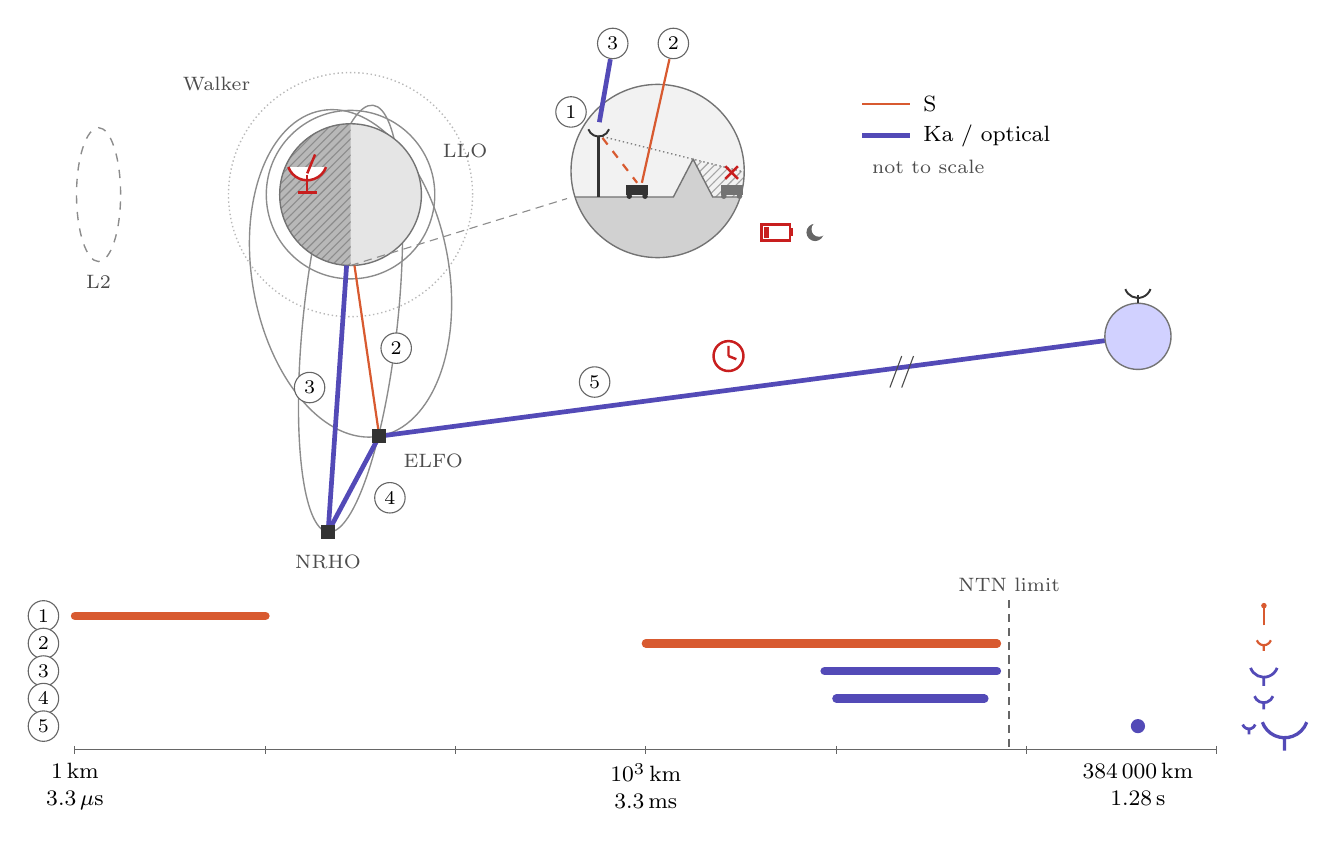
\begin{tikzpicture}[x=1cm,y=1cm, font=\footnotesize,
  lowband/.style={draw=lowc, line width=0.8pt},
  highband/.style={draw=highc, line width=1.7pt},
  orbit/.style={draw=black!45, line width=0.5pt},
  num/.style={circle, draw=black!60, fill=white, inner sep=0.6pt, minimum size=11pt, font=\scriptsize},
  sat/.style={fill=black!80, minimum size=5pt, inner sep=0pt, rectangle},
  lab/.style={font=\scriptsize, text=black!70},
  flag/.style={draw=accent, line width=0.9pt},
]
% ================= SCENE =================
% ---- L2 halo behind the far side ----
\draw[orbit, dashed] (1.3,4.0) ellipse (0.28 and 0.85);
\node[lab, anchor=north] at (1.3,3.1) {L2};
% ---- Walker (medium circular orbit) ----
\draw[draw=black!28, line width=0.5pt, densely dotted] (4.5,4.0) circle (1.55);
\node[lab, anchor=south east] at (3.35,5.2) {Walker};
% ---- ELFO and NRHO, apolune below the south pole ----
\draw[orbit, rotate around={10:(4.5,3.0)}] (4.5,3.0) ellipse (1.25 and 2.1);
\draw[orbit, rotate around={-6:(4.5,2.425)}] (4.5,2.425) ellipse (0.6 and 2.725);
% ---- Moon: near side lit (towards Earth), far side shaded and hatched ----
\fill[black!10] (4.5,4.0) circle (0.9);
\fill[black!28] (4.5,4.9) arc (90:270:0.9) -- cycle;
\fill[pattern=north east lines, pattern color=black!45] (4.5,4.9) arc (90:270:0.9) -- cycle;
\draw[black!55, line width=0.5pt] (4.5,4.0) circle (0.9);
% ---- LLO ----
\draw[orbit] (4.5,4.0) circle (1.07);
\node[lab, anchor=west] at (5.55,4.55) {LLO};
% ---- radio telescope on the far side (Shielded Zone) ----
\begin{scope}[shift={(3.95,4.25)}]
  \fill[white] (-0.24,0.10) arc (200:340:0.255) -- cycle;
  \draw[flag] (-0.24,0.10) arc (200:340:0.255);
  \draw[flag] (0,0.0) -- (0,-0.22) (-0.12,-0.22) -- (0.12,-0.22);
  \draw[flag] (0,0.02) -- (0.10,0.26);
\end{scope}
% ---- relays at apolune, Earth ----
\coordinate (SP)   at (4.5,3.1);
\coordinate (ELFO) at (4.865,0.932);
\coordinate (NRHO) at (4.215,-0.285);
\coordinate (EARTH) at (14.5,2.2);
\draw[lowband]  ($(SP)+(0.05,0)$) -- (ELFO);                 % 2
\draw[highband] ($(SP)+(-0.05,0)$) -- (NRHO);                % 3
\draw[highband] (ELFO) -- (NRHO);                            % 4
\draw[highband] (ELFO) -- ($(EARTH)+(-0.42,-0.055)$);        % 5
\node[sat] at (ELFO) {};
\node[sat] at (NRHO) {};
\node[lab, anchor=west] at (5.05,0.62) {ELFO};
\node[lab, anchor=north] at (4.215,-0.45) {NRHO};
\draw[black!70] (11.35,1.55) -- (11.5,1.95); \draw[black!70] (11.5,1.55) -- (11.65,1.95);
% ---- clock on the trunk (delay) ----
\begin{scope}[shift={(9.3,1.95)}]
  \draw[flag, fill=white] (0,0) circle (0.19);
  \draw[flag] (0,0) -- (0,0.13) (0,0) -- (0.10,-0.04);
\end{scope}
% ---- Earth with a DSN dish ----
\fill[blue!18] (EARTH) circle (0.42); \draw[black!55, line width=0.5pt] (EARTH) circle (0.42);
\begin{scope}[shift={(14.5,2.72)}]
  \draw[black!80, line width=0.7pt] (-0.16,0.08) arc (200:340:0.17);
  \draw[black!80, line width=0.7pt] (0,0) -- (0,-0.10);
\end{scope}
% ---- link numbers in the scene ----
\node[num] at (5.08,2.05) {2};
\node[num] at (3.98,1.55) {3};
\node[num] at (5.0,0.15) {4};
\node[num] at (7.6,1.62) {5};
% ---- south-polar surface inset ----
\draw[black!45, densely dashed, line width=0.4pt] (SP) -- (7.25,3.95);
\begin{scope}
  \clip (8.4,4.3) circle (1.1);
  \fill[black!5] (8.4,4.3) circle (1.1);
  \fill[pattern=north east lines, pattern color=black!35] (8.85,4.45) -- (9.6,4.2625) -- (9.6,3.97) -- (9.1,3.97) -- cycle;
  \fill[black!18] (7.2,3.97) -- (8.6,3.97) -- (8.85,4.45) -- (9.1,3.97) -- (9.6,3.97) -- (9.6,3.1) -- (7.2,3.1) -- cycle;
  \draw[black!55, line width=0.5pt] (7.2,3.97) -- (8.6,3.97) -- (8.85,4.45) -- (9.1,3.97) -- (9.6,3.97);
  \draw[black!50, densely dotted, line width=0.5pt] (7.65,4.75) -- (9.6,4.2625);
\end{scope}
\draw[black!55, line width=0.5pt] (8.4,4.3) circle (1.1);
\draw[black!80, line width=0.9pt] (7.65,3.97) -- (7.65,4.75);                 % gateway mast
\draw[black!80, line width=0.7pt] (7.52,4.83) arc (200:340:0.14);              % gateway dish
\fill[black!80] (8.0,4.0) rectangle (8.28,4.12);                               % rover in view
\fill[black!80] (8.04,3.98) circle (0.035) (8.24,3.98) circle (0.035);
\fill[black!55] (9.2,4.0) rectangle (9.48,4.12);                               % rover in shadow
\fill[black!55] (9.24,3.98) circle (0.035) (9.44,3.98) circle (0.035);
\draw[flag] (9.26,4.20) -- (9.42,4.36) (9.26,4.36) -- (9.42,4.20);              % no line of sight
\draw[lowband, dashed] (7.7,4.72) -- (8.14,4.15);                              % 1
\node[num] at (7.30,5.05) {1};
\draw[highband] (7.66,4.92) -- (7.80,5.72);  \node[num] at (7.83,5.92) {3};    % 3 from the gateway
\draw[lowband] (8.20,4.15) -- (8.55,5.72);   \node[num] at (8.60,5.92) {2};    % 2 from the rover
% ---- battery and crescent: power through the lunar night ----
\draw[flag] (9.72,3.42) rectangle (10.08,3.62); \fill[accent] (10.08,3.47) rectangle (10.12,3.57);
\fill[accent] (9.75,3.45) rectangle (9.82,3.59);
\fill[black!60] (10.40,3.52) circle (0.11); \fill[white] (10.45,3.56) circle (0.095);
% ---- legend (band only) ----
\draw[lowband]  (11.0,5.15) -- (11.6,5.15); \node[anchor=west] at (11.65,5.15) {S};
\draw[highband] (11.0,4.75) -- (11.6,4.75); \node[anchor=west] at (11.65,4.75) {Ka / optical};
\node[lab, anchor=west] at (11.0,4.35) {not to scale};
% ================= STRIP: slant range and one-way delay (log scale) =================
% x = 1 + 2.4167*log10(R/km)
\foreach \y/\n in {-1.35/1,-1.7/2,-2.05/3,-2.4/4,-2.75/5} \node[num] at (0.6,\y) {\n};
\draw[lowc,  line width=3pt, line cap=round] (1.0,-1.35) -- (3.42,-1.35);
\draw[lowc,  line width=3pt, line cap=round] (8.25,-1.7) -- (12.71,-1.7);
\draw[highc, line width=3pt, line cap=round] (10.52,-2.05) -- (12.71,-2.05);
\draw[highc, line width=3pt, line cap=round] (10.67,-2.4) -- (12.55,-2.4);
\fill[highc] (14.5,-2.75) circle (0.09);
\draw[black!60] (1.0,-3.05) -- (15.5,-3.05);
\foreach \d in {0,...,6} \draw[black!60] ({1+2.4167*\d},-3.0) -- ({1+2.4167*\d},-3.1);
\node[anchor=north, align=center] at (1.0,-3.1)  {1\,km\\3.3\,$\mu$s};
\node[anchor=north, align=center] at (8.25,-3.1) {$10^3$\,km\\3.3\,ms};
\node[anchor=north, align=center] at (14.5,-3.1) {384\,000\,km\\1.28\,s};
% 3GPP NTN one-way delay limit (270.73 ms, about 81 000 km)
\draw[black!60, densely dashed, line width=0.6pt] (12.865,-1.15) -- (12.865,-3.05);
\node[lab, anchor=south] at (12.865,-1.17) {NTN limit};
% ---- relative aperture of each link, drawn as antennas (colour = band) ----
\draw[lowc, line width=0.9pt] (16.1,-1.47) -- (16.1,-1.24); \fill[lowc] (16.1,-1.22) circle (0.035);   % omni
\draw[lowc, line width=0.8pt] (16.01,-1.66) arc (200:340:0.095) (16.099,-1.723) -- (16.099,-1.795);                                       % 0.5 m
\draw[highc, line width=1.0pt] (15.93,-2.01) arc (200:340:0.18) (16.099,-2.128) -- (16.099,-2.239);                                       % 1.5 m
\draw[highc, line width=1.0pt] (15.98,-2.37) arc (200:340:0.125) (16.097,-2.452) -- (16.097,-2.538);                                      % 1 m
\draw[highc, line width=1.0pt] (15.83,-2.73) arc (200:340:0.085) (15.910,-2.786) -- (15.910,-2.854);                                      % 0.75 m
\draw[highc, line width=1.2pt] (16.08,-2.70) arc (200:340:0.30) (16.362,-2.897) -- (16.362,-3.062);                                       % 34 m
\end{tikzpicture}

% Previous, text-labelled TikZ version: % Overview figure: geometry (top) and slant-range / delay strip (bottom). Not to scale.
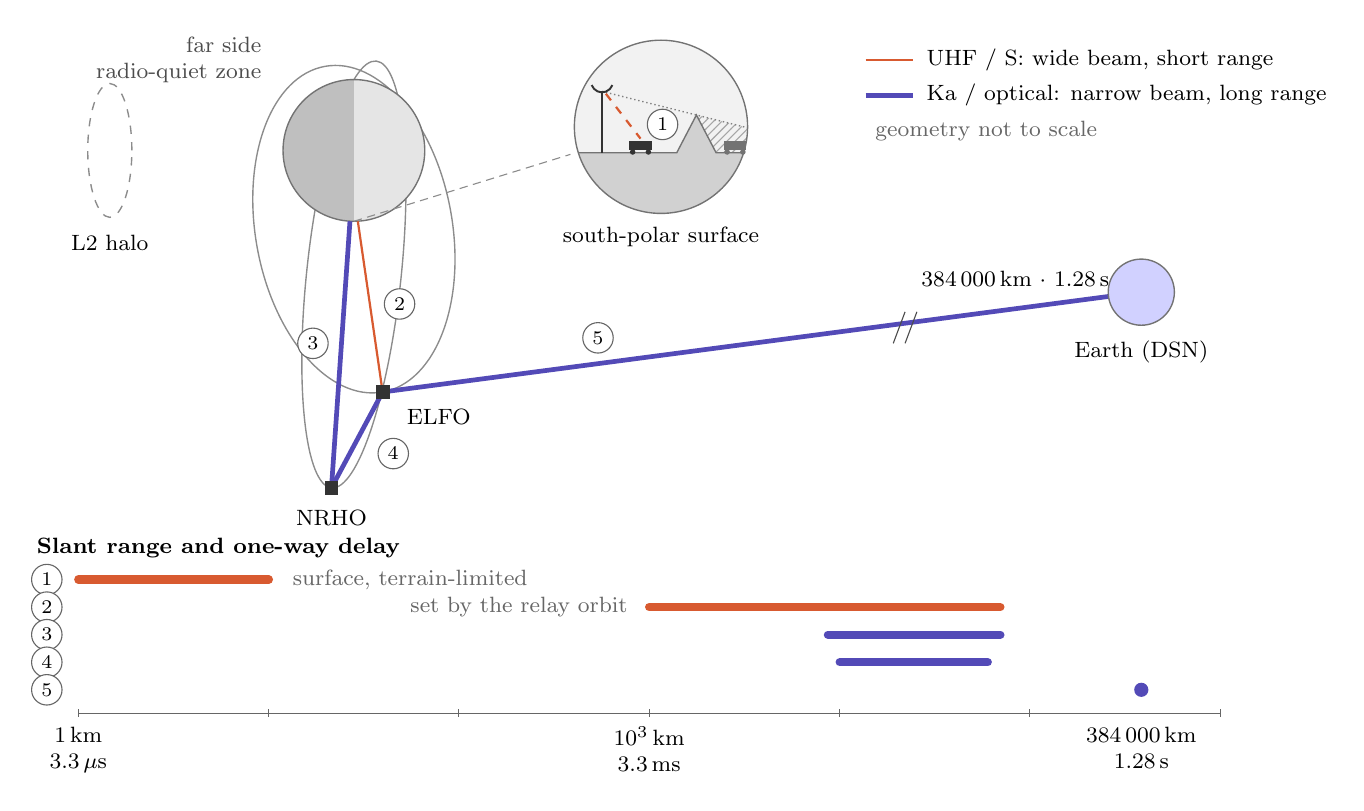
\begin{tikzpicture}[x=1cm,y=1cm, font=\footnotesize,
  lowband/.style={draw=lowc, line width=0.8pt},
  highband/.style={draw=highc, line width=1.7pt},
  orbit/.style={draw=black!45, line width=0.5pt},
  num/.style={circle, draw=black!60, fill=white, inner sep=0.6pt, minimum size=11pt, font=\scriptsize},
  sat/.style={fill=black!80, minimum size=5pt, inner sep=0pt, rectangle},
]
% ---------- far side, L2 halo ----------
\draw[orbit, dashed] (1.4,4.0) ellipse (0.28 and 0.85);
\node[anchor=north] at (1.4,3.05) {L2 halo};
% ---------- orbits (apolune below the south pole) ----------
\draw[orbit, rotate around={10:(4.5,3.0)}] (4.5,3.0) ellipse (1.25 and 2.1);
\draw[orbit, rotate around={-6:(4.5,2.425)}] (4.5,2.425) ellipse (0.6 and 2.725);
% ---------- Moon ----------
\fill[black!10] (4.5,4.0) circle (0.9);
\fill[black!25] (4.5,4.9) arc (90:270:0.9) -- cycle;   % far side (away from Earth)
\draw[black!55, line width=0.5pt] (4.5,4.0) circle (0.9);
\node[align=right, anchor=east, text=black!70] at (3.45,5.15) {far side\\radio-quiet zone};
% ---------- relays at apolune ----------
\coordinate (SP)   at (4.5,3.1);
\coordinate (ELFO) at (4.865,0.932);
\coordinate (NRHO) at (4.215,-0.285);
\coordinate (EARTH) at (14.5,2.2);
% ---------- links ----------
\draw[lowband]  ($(SP)+(0.05,0)$) -- (ELFO);                 % 2 surface-to-relay
\draw[highband] ($(SP)+(-0.05,0)$) -- (NRHO);                % 3 gateway backhaul
\draw[highband] (ELFO) -- (NRHO);                            % 4 inter-satellite
\draw[highband] (ELFO) -- ($(EARTH)+(-0.42,-0.055)$);        % 5 trunk
\node[sat] at (ELFO) {};
\node[sat] at (NRHO) {};
\node[anchor=west] at (5.05,0.62) {ELFO};
\node[anchor=north] at (4.215,-0.45) {NRHO};
% break on the trunk + distance
\draw[black!70] (11.35,1.55) -- (11.5,1.95); \draw[black!70] (11.5,1.55) -- (11.65,1.95);
\node[anchor=south] at (12.9,2.15) {384\,000\,km $\cdot$ 1.28\,s};
% ---------- Earth ----------
\fill[blue!18] (EARTH) circle (0.42); \draw[black!55, line width=0.5pt] (EARTH) circle (0.42);
\node[anchor=north] at (14.5,1.7) {Earth (DSN)};
% ---------- link numbers ----------
\node[num] at (5.08,2.05) {2};
\node[num] at (3.98,1.55) {3};
\node[num] at (5.0,0.15) {4};
\node[num] at (7.6,1.62) {5};
% ---------- south-polar surface inset ----------
\draw[black!45, densely dashed, line width=0.4pt] (SP) -- (7.25,3.95);
\begin{scope}
  \clip (8.4,4.3) circle (1.1);
  \fill[black!5] (8.4,4.3) circle (1.1);
  % radio shadow behind the ridge, bounded by the grazing line of sight
  \fill[pattern=north east lines, pattern color=black!35] (8.85,4.45) -- (9.6,4.2625) -- (9.6,3.97) -- (9.1,3.97) -- cycle;
  \fill[black!18] (7.2,3.97) -- (8.6,3.97) -- (8.85,4.45) -- (9.1,3.97) -- (9.6,3.97) -- (9.6,3.1) -- (7.2,3.1) -- cycle;
  \draw[black!55, line width=0.5pt] (7.2,3.97) -- (8.6,3.97) -- (8.85,4.45) -- (9.1,3.97) -- (9.6,3.97);
  \draw[black!50, densely dotted, line width=0.5pt] (7.65,4.75) -- (9.6,4.2625);   % grazing line of sight
\end{scope}
\draw[black!55, line width=0.5pt] (8.4,4.3) circle (1.1);
% gateway mast and dish
\draw[black!80, line width=0.9pt] (7.65,3.97) -- (7.65,4.75);
\draw[black!80, line width=0.7pt] (7.52,4.83) arc (200:340:0.14);
% rover in coverage
\fill[black!80] (8.0,4.0) rectangle (8.28,4.12);
\fill[black!80] (8.04,3.98) circle (0.035) (8.24,3.98) circle (0.035);
% rover in the terrain shadow (no line of sight)
\fill[black!55] (9.2,4.0) rectangle (9.48,4.12);
\fill[black!55] (9.24,3.98) circle (0.035) (9.44,3.98) circle (0.035);
\draw[lowband, dashed] (7.7,4.72) -- (8.14,4.15);            % 1 surface access
\node[num] at (8.42,4.33) {1};
\node[anchor=north] at (8.4,3.15) {south-polar surface};
% ---------- legend ----------
\draw[lowband]  (11.0,5.15) -- (11.6,5.15); \node[anchor=west] at (11.65,5.15) {UHF / S: wide beam, short range};
\draw[highband] (11.0,4.7)  -- (11.6,4.7);  \node[anchor=west] at (11.65,4.7)  {Ka / optical: narrow beam, long range};
\node[anchor=west, text=black!60] at (11.0,4.25) {geometry not to scale};
% ---------- slant-range and delay strip (log scale) ----------
% x = 1 + 2.4167*log10(R/km), 1 km .. 10^6 km
\node[anchor=west] at (0.35,-1.05) {\textbf{Slant range and one-way delay}};
\foreach \y/\n in {-1.45/1,-1.8/2,-2.15/3,-2.5/4,-2.85/5} \node[num] at (0.6,\y) {\n};
\draw[lowc,  line width=3pt, line cap=round] (1.0,-1.45) -- (3.42,-1.45);
\draw[lowc,  line width=3pt, line cap=round] (8.25,-1.8) -- (12.71,-1.8);
\draw[highc, line width=3pt, line cap=round] (10.52,-2.15) -- (12.71,-2.15);
\draw[highc, line width=3pt, line cap=round] (10.67,-2.5) -- (12.55,-2.5);
\fill[highc] (14.5,-2.85) circle (0.09);
\draw[black!60] (1.0,-3.15) -- (15.5,-3.15);
\foreach \d in {0,...,6} \draw[black!60] ({1+2.4167*\d},-3.1) -- ({1+2.4167*\d},-3.2);
\node[anchor=north, align=center] at (1.0,-3.2)    {1\,km\\3.3\,$\mu$s};
\node[anchor=north, align=center] at (8.25,-3.2)   {$10^3$\,km\\3.3\,ms};
\node[anchor=north, align=center] at (14.5,-3.2)   {384\,000\,km\\1.28\,s};
\node[anchor=west, text=black!60] at (3.6,-1.45)   {surface, terrain-limited};
\node[anchor=east, text=black!60] at (8.1,-1.8)    {set by the relay orbit};
\end{tikzpicture}

% Rendered raster version of the same figure (1448x1086 px, below 300 dpi at this width):
% 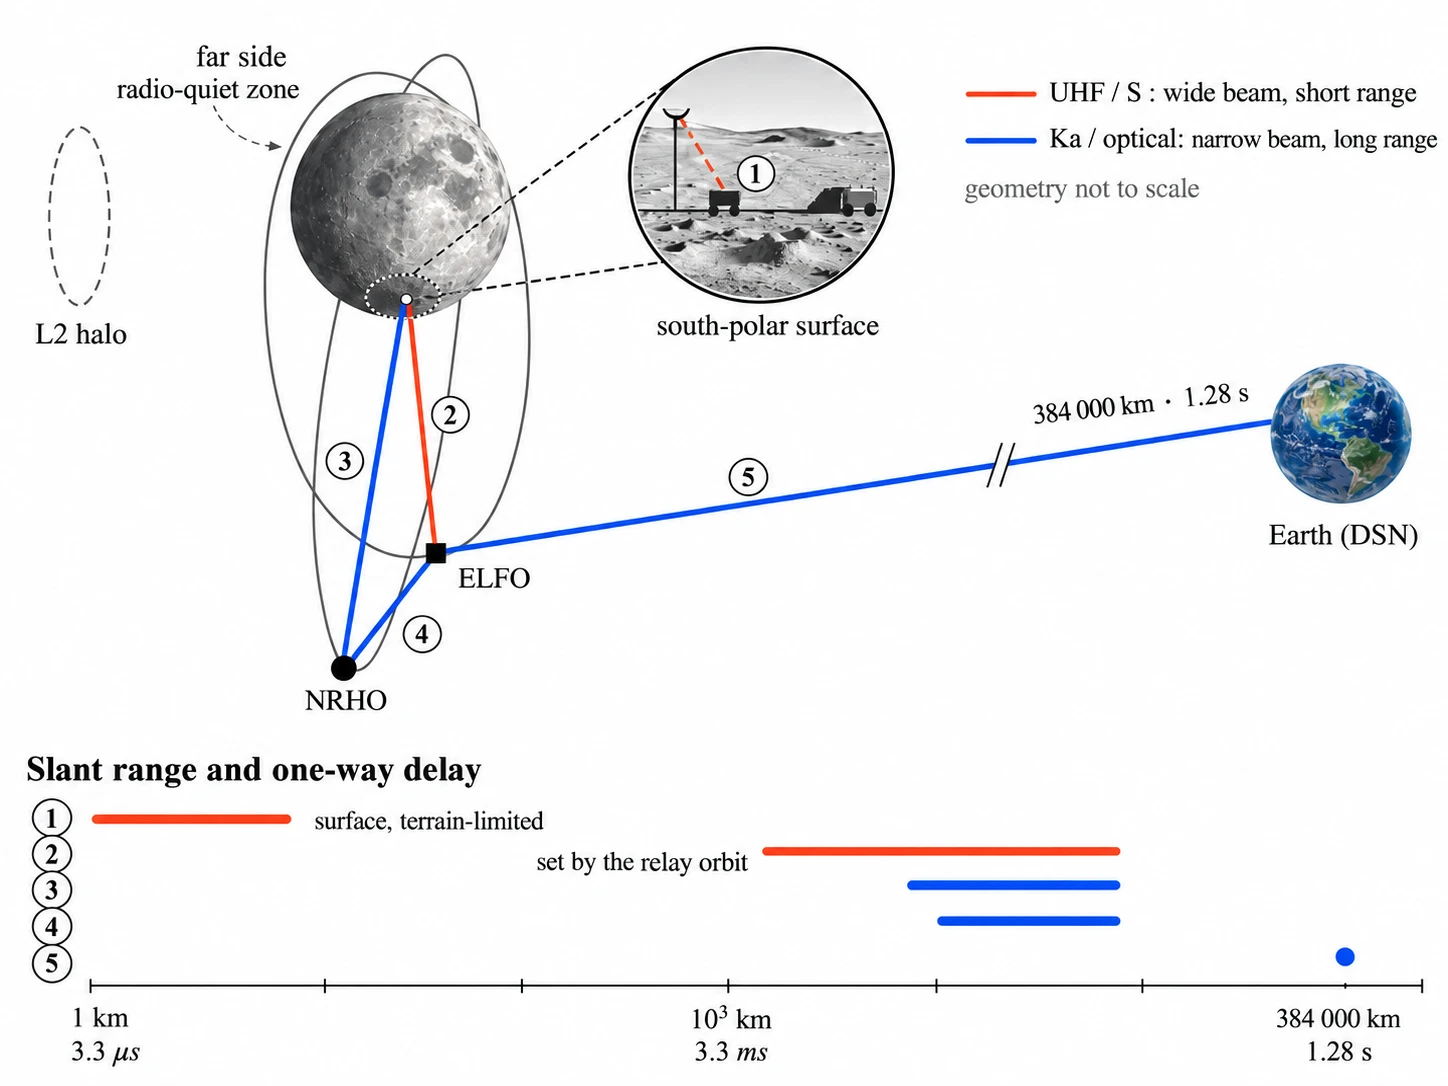
\includegraphics[width=0.94\textwidth]{figs/fig_overview.png}
\caption{Lunar communication chain and roadmap of the tutorial (not to scale). The relay orbit sets the slant range of each link, and range, band and data rate set its aperture; red icons mark where terrestrial assumptions fail on the Moon.}
\label{fig:overview}
\end{figure*}

\IEEEPARstart{L}{unar} communications infrastructure is under active development by several national space agencies and commercial providers. NASA's Lunar Communications Relay and Navigation Systems (LCRNS) project aims to establish a commercial lunar communications and navigation service~\cite{lcrns_esper2025}, and in 2024 NASA awarded Intuitive Machines a Near Space Network contract for lunar relay services that include position, navigation and timing~\cite{nasa_im_contract}. The Moonlight program of the European Space Agency plans a constellation of five satellites, one for communications and four for navigation, with initial operations by the end of 2028 and full operations by 2030~\cite{esa_moonlight_overview,esa_moonlight_csc}. China has deployed two relay satellites beyond Earth orbit, Queqiao in 2018 and Queqiao-2 in 2024; Queqiao has exceeded its design lifetime, and Queqiao-2 has taken over the relay service for Chang'e-4 and supports the Chang'e-6 to Chang'e-8 missions~\cite{chen_ce4_relay,cnsa_queqiao2}. A 2022 survey identified 106 planned cislunar and lunar missions from 19~nations and ESA~\cite{csis_fly_me_moon}.

For communications engineers accustomed to terrestrial or Earth-orbit satellite systems, the lunar environment differs in several respects that affect link design. Slant ranges span from a few kilometers for surface-to-surface links to \SI{384000}{km} for the Earth--Moon trunk, a spread of five orders of magnitude within a single network. The Earth--Moon round-trip time of \SI{2.56}{\second} exceeds the design assumptions of standard TCP, of 5G~NR hybrid automatic repeat request on the trunk link, and of online certificate validation. Surface nodes must operate through a lunar night of \SI{14.77}{days}, which constrains power availability and causes the network topology to vary over the lunar day. The Shielded Zone of the Moon covers the part of the far side lying more than \SI{23.2}{\degree} beyond the mean limb, together with an adjacent volume of space. No.~22.22 of the Radio Regulations protects it for radio astronomy and other passive services, and active services may transmit within it only in the bands exempted by Nos.~22.23 and~22.24, which inverts the usual regulatory relationship between active communications services and passive services.

For every link that terminates on a relay satellite, the slant range, which is the dominant term of the free-space path loss, is determined by orbital mechanics. The relay orbit determines the range, and the range in turn determines the antenna aperture required to deliver a given data rate at a given carrier frequency. This relationship, referred to in what follows as the aperture-range scaling, is the organizing principle of this tutorial. The paper derives it from first principles, applies it to a representative worked example, and generalizes it through parametric analysis.
\subsection{Related Review Articles}
The lunar communications literature is fragmented across subdomains. Marine-Roig and Baeza~\cite{marine_roig_survey} present a systematic review of lunar communication and navigation systems that follows the PRISMA methodology, covers 175~publications across seven research domains, and proposes an integrated architectural roadmap. Serria \emph{et al.}~\cite{alqodah_review} review lunar surface communication and the antennas used in lunar missions and research, assessed against propagation and radiation effects. Elewaily \emph{et al.}~\cite{islam_dtn_survey} survey delay-tolerant networking for deep-space relay networks, and Liyanaarachchi \emph{et al.}~\cite{liyanaarachchi_cislunar} examine which 6G concepts carry over to cislunar networks. Jamshed \emph{et al.}~\cite{jamshed_ntn_tutorial} and Nguyen \emph{et al.}~\cite{nguyen_ntn_ojcoms2024} treat non-terrestrial networks in the broader satellite-aerial context. Caini and de~Cola~\cite{e2e_vs_dtn_2026} compare end-to-end TCP and QUIC with DTN over QUICCL/LTP on a common Earth--Moon testbed. The lunar surveys among these works catalog what has been proposed and flown, and the non-terrestrial network tutorials address Earth-orbit and aerial platforms. None of them derives the aperture values and data rates of lunar links from the link equation, so the physical relationship between orbit selection, aperture, pointing, and power remains implicit. The present paper makes that relationship explicit through a scaling law derived from first principles. The law enables system-level trade-offs (orbit versus aperture, frequency versus pointing, data rate versus spacecraft power) that the mission-specific literature does not address. The closest methodological antecedent is Saeed \emph{et al.}~\cite{saeed_ojcoms2021}, who state the radio-frequency and optical link-budget equations for satellite-to-satellite links in integrated satellite-aerial networks and plot the received power and $E_b/N_0$ against link distance. The present paper extends that approach to the lunar domain. There, the five-orders-of-magnitude span in slant range and the orbital-mechanics constraint on aperture introduce a coupling that the satellite-aerial case does not exhibit, and the terrestrial design assumptions that the satellite-aerial case preserves (continuous connectivity, online authentication, fading-based handover) cease to hold at identifiable numerical thresholds.

\subsection{Contributions}
The contributions of this paper are fourfold.
\begin{enumerate}
\item It derives the aperture-range scaling law from the link equation, showing that the required aperture product scales linearly with slant range and wavelength and as the square root of the data rate, so that for links to a relay the orbit becomes the design decision from which aperture, pointing and frequency follow.
\item It illustrates the method with a canonical Ka-band trunk budget, with all parameters in a single table, and generalizes it through parametric curves to five canonical lunar links, each characterized by its dominant constraint.
\item It surveys the terrestrial assumptions that cease to hold on the Moon and the numerical thresholds at which they fail, for protocol timers, handover, power, security and spectrum.
\item It reduces the design guidance to a decision-flow procedure and a terminology map, and states the open research problems as deliverables tied to the sections that motivate them.
\end{enumerate}

\subsection{Terminology Bridge}
An engineer trained on terrestrial cellular systems already has a name for every element of a lunar network, but the assumptions behind those names do not all transfer. Table~\ref{tab:terminology} lists the concepts for which the transfer is least reliable and states, for each, the specific assumption that fails. Terms whose definition carries over unchanged are omitted. The entries are ordered from the access network to spectrum regulation, and each points to the section in which the failure is quantified. Two further mappings are deferred to the sections in which their subject matter is treated: radio-layer mechanisms in deep-space against 3GPP practice in Section~\ref{sec:assets}, and the vocabularies of the three standards families that jointly govern a lunar network in Section~\ref{sec:protocol}.

\begin{table*}[!t]
\caption{Terrestrial Concepts Whose Underlying Assumptions Fail on the Moon}
\label{tab:terminology}
\centering
\footnotesize
\begin{tabularx}{\textwidth}{@{}>{\raggedright\arraybackslash}p{2.4cm}>{\raggedright\arraybackslash}p{4.1cm}>{\raggedright\arraybackslash}X@{}}
\toprule
Terrestrial concept & Lunar counterpart & Assumption that fails \\
\midrule
User equipment & Rover, EVA suit, emplaced instrument & The user population comprises crewed EVA with multi-camera video, teleoperated and autonomous rovers, and fixed science instruments, with requirements that range from continuous low-latency control links of a few hundred kbit/s to bulk returns of several gigabytes per day, so no single terminal profile applies (\S\ref{sec:capacity}) \\
Base station & Lander, deployed mast, or relay satellite & The role is transient and power-limited; for a lander or mast the coverage is bounded by terrain and mast height, and for a relay satellite the served range follows from the relay orbit (\S\ref{sec:capacity}, \S\ref{sec:ntn}) \\
Core network & Local surface core, or an Earth-side core \SI{1.28}{\second} away & A co-located, always-reachable core cannot be assumed, which forces either local termination or store-and-forward operation (\S\ref{sec:protocol}) \\
Backhaul & Trunk link to Earth & No wireline exists: the backhaul is a wireless link, limited by aperture and pointing from the surface gateway to the relay and by weather and ground-station scheduling on the trunk to Earth (\S\ref{sec:worked}, \S\ref{sec:parametric}) \\
Cell & Coverage cell & Terrain rather than interference sets the boundary, so frequency reuse is not the binding constraint and the planning tool is a ray tracer over an elevation model (\S\ref{sec:capacity}) \\
Handover & Handover within planned overlap & The serving signal holds at full strength until the ridge occludes it, so the measured signal gives no warning; handover must be scheduled from a terrain-based visibility prediction and the overlap sized from terrain geometry, and where the deployment provides no overlap the rover buffers traffic until the next contact (\S\ref{sec:capacity}) \\
HARQ and ARQ & Retransmission terminated at the relay & Terrestrial HARQ timing is exceeded on any relay service link, and the NTN scheduling offsets and per-process HARQ disabling absorb the relay range but not the \SI{2.56}{\second} round trip to Earth, so reliability must be restored hop by hop, by LTP or bundle-layer retransmission on the long-delay segment (\S\ref{sec:protocol}) \\
GNSS & Lunar PNT service & Earth GNSS signals are weak but usable on the near side and in lunar orbit, as LuGRE and the relay GNSS receivers show, whereas no Earth constellation is visible from the far side, where position and time must be supplied by the lunar relay constellation (\S\ref{sec:pnt}) \\
Spectrum license & ITU-R allocation and Shielded Zone protection & Within the Shielded Zone, No.~22.22 of the Radio Regulations prohibits emissions causing harmful interference to radio astronomy and other passive services except in the bands exempted by Nos.~22.23 and~22.24, so the passive services are the protected party and active emitters are confined to the exempted bands (\S\ref{sec:spectrum}) \\
\bottomrule
\end{tabularx}
\end{table*}

\begin{table*}[!t]
\caption{Acronyms}
\label{tab:acronyms}
\centering
\footnotesize
\begin{tabularx}{\textwidth}{@{}lXlX@{}}
\toprule
Acronym & Definition & Acronym & Definition \\
\midrule
3GPP & 3rd Generation Partnership Project & LLO & Low lunar orbit \\
ARQ & Automatic repeat request & LRO & Lunar Reconnaissance Orbiter \\
BPSec & Bundle Protocol Security & LTE & Long Term Evolution \\
BPSK & Binary phase-shift keying & LTP & Licklider Transmission Protocol \\
BPv7 & Bundle Protocol version 7 & MIMO & Multiple-input multiple-output \\
CCSDS & Consultative Committee for Space Data Systems & NR & New Radio \\
CGR & Contact Graph Routing & NRHO & Near-rectilinear halo orbit \\
COP-1 & Communications Operation Procedure-1 & NTN & Non-terrestrial network \\
COSE & CBOR Object Signing and Encryption & OCSP & Online Certificate Status Protocol \\
DSN & Deep Space Network & PKI & Public-key infrastructure \\
DTN & Delay-tolerant networking & PNT & Position, navigation and timing \\
EIRP & Equivalent isotropically radiated power & PRS & Positioning reference signal \\
ELFO & Elliptical lunar frozen orbit & QPSK & Quadrature phase-shift keying \\
EVA & Extravehicular activity & RF & Radio frequency \\
GDOP & Geometric dilution of precision & RIS & Reconfigurable intelligent surface \\
GNSS & Global navigation satellite system & RTT & Round-trip time \\
GPS & Global Positioning System & SFCG & Space Frequency Coordination Group \\
HARQ & Hybrid automatic repeat request & TBR & To be resolved \\
ITU-R & ITU Radiocommunication Sector & TCP & Transmission Control Protocol \\
KPLO & Korea Pathfinder Lunar Orbiter & UHF & Ultra high frequency \\
LCRNS & Lunar Communications Relay and Navigation Systems & WRC & World Radiocommunication Conference \\
LLCD & Lunar Laser Communication Demonstration &  &  \\
\bottomrule
\end{tabularx}
\end{table*}

\subsection{Paper Organization}
Fig.~\ref{fig:overview} provides a map of the material that follows. The five orbit families compared in Section~\ref{sec:pnt} surround the Moon, each drawn in its own color and labelled with the systems of Section~\ref{sec:assets} that use it: low lunar orbit (LRO, KPLO), the elliptical frozen orbit (LCRNS, Moonlight), the near-rectilinear halo orbit (Gateway), the Earth--Moon L2 halo orbit, drawn as seen from Earth: Queqiao circles the L2 point behind the far side on a ring larger than the lunar disc, so it is never hidden by the Moon and can relay the far side, which has no line of sight to Earth, and Walker constellations, shown as several orbital planes. The relay orbits fix the slant ranges of the links they serve, which is the starting point of the link analysis in Sections~\ref{sec:fundamentals} to~\ref{sec:parametric}, and the five numbered links are those sized in Section~\ref{sec:parametric}; line color gives the band, and in the south-polar inset links~2 and~3 leave from the rover at S-band and from the surface gateway at Ka-band. The south-polar inset illustrates the terrain shadowing that governs surface coverage and handover, treated in Section~\ref{sec:capacity}, while the placement of the relays at apolune over the pole anticipates the constellation and navigation geometry of Section~\ref{sec:pnt}. The lower strip spans five orders of magnitude in slant range and in one-way delay and draws the relative aperture of each link, which follows from its range, carrier frequency and data rate through the aperture-range scaling of Section~\ref{sec:fundamentals}; the dashed line at the one-way delay limit of 3GPP non-terrestrial networks separates the relay links from the trunk to Earth and motivates the protocol analysis of Sections~\ref{sec:ntn} and~\ref{sec:protocol}. The red icons locate the four terrestrial assumptions that fail on the Moon: the delay on the trunk (Sections~\ref{sec:ntn} and~\ref{sec:protocol}), terrain blocking at the surface (Section~\ref{sec:capacity}), and the lunar night and the far-side Shielded Zone (Section~\ref{sec:spectrum}).

In order of presentation, Section~\ref{sec:assets} inventories the assets that have flown or are under contract and compares the radio practice of deep-space and 3GPP systems. Section~\ref{sec:fundamentals} derives the link equation and the aperture-range scaling. Section~\ref{sec:worked} presents the canonical worked example. Section~\ref{sec:parametric} generalizes the result through parametric curves and introduces the five canonical lunar links. Section~\ref{sec:environment} summarizes the environmental constraints. Section~\ref{sec:guidelines} states the design guidelines and the decision-flow procedure. Sections~\ref{sec:capacity} through~\ref{sec:spectrum} survey capacity and mobility, constellation design and position-navigation-timing, the transfer of 3GPP non-terrestrial network concepts, protocol design for intermittent links, and security, power and spectrum. Section~\ref{sec:measurement} discusses the measurement gap, Section~\ref{sec:open} presents future research directions, and Section~\ref{sec:conclusion} concludes. Table~\ref{tab:acronyms} lists the acronyms used in the paper.
\section{Lunar Communication Assets Today}
\label{sec:assets}

This section reviews the lunar communication systems that have flown or are under contract and lists, for each, the four quantities that enter a link budget: orbit, band, aperture and delivered rate (Table~\ref{tab:assets}). Two observations follow from it. Every asset flown to date operates as a scheduled point-to-point link rather than as a network, with capacity allocated by a plan generated on Earth and no autonomous routing on board. The aperture and band of each asset also depend on its orbit, a dependence derived in Section~\ref{sec:fundamentals}.

\begin{table*}[!t]
\caption{Lunar Communication Assets Flown, Operating or Under Contract}
\label{tab:assets}
\centering
\footnotesize
\begin{tabularx}{\textwidth}{@{}>{\raggedright\arraybackslash}p{2.7cm}>{\raggedright\arraybackslash}p{3.5cm}>{\raggedright\arraybackslash}p{3.4cm}>{\raggedright\arraybackslash}p{1.8cm}>{\raggedright\arraybackslash}X@{}}
\toprule
Asset & Orbit or location & Bands & Aperture & Rate delivered or specified \\
\midrule
\multicolumn{5}{@{}l}{\emph{Relays and orbiters, flown or operating}}\\
Queqiao~\cite{chen_ce4_relay,queqiao_relay_review_2021} & Earth--Moon L2 halo & X to surface, S to Earth (X backup) & \SI{4.2}{m} & \SI{125}{bps} forward, up to \SI{555}{kbps} return (lander); \SI{2}{}--\SI{4}{Mbps} S to Earth (X backup over \SI{10}{Mbps}) \\
Queqiao-2~\cite{cnsa_queqiao2,planetary_queqiao2,hong_lovex_2026,lei_queqiao2_data_2026} & Elliptical frozen, period \SI{24}{hours} (\SI{12}{hours} planned) & X to surface, S and Ka to Earth & \SI{4.2}{m}; \SI{0.6}{m} S/Ka & Up to \SI{500}{Mbps} Ka to Earth; surface-link rates not published \\
LRO~\cite{lro_ka_analysis} & Polar, \SI{50}{km} (to 2011), then ${\approx}\SI{30}{}\times\SI{180}{km}$ & S \SI{2.2}{GHz}, Ka \SI{25.65}{GHz} & \SI{0.75}{m} & \SI{100}{Mbps} Ka downlink \\
KPLO~\cite{kim_kplo_dtn} & Polar, \SI{100}{km} & S, X & --- & \SI{8.5}{Mbps} X downlink; delay-tolerant payload \\
\addlinespace[2pt]
\multicolumn{5}{@{}l}{\emph{Relay and navigation systems, planned or under contract}}\\
Gateway~\cite{gateway_comm} & NRHO & S, X, Ka, optical & \SI{1}{m}; \SI{1.25}{m} & \SI{16}{Mbps} forward, \SI{40}{Mbps} return on the lunar link \\
LCRNS~\cite{lcrns_ref_const,nasa_lunar_relay_srd} & Five ELFOs, period near \SI{30}{hours} & S, Ka to users; X, Ka to Earth; optical (TBR) & --- & \SI{1}{}--\SI{50}{Mbps} Ka \\
Moonlight~\cite{esa_moonlight_overview,telespazio_moonlight,telespazio_moonlight_web} & One communications ELFO at \SI{12}{hours}, four navigation ELFOs at \SI{24}{hours} & S, K to users; Earth link not published & --- & Not published \\
Lunar Pathfinder~\cite{sstl_pathfinder_guide,sstl_pathfinder_mission,esa_pathfinder_2026} & ELFO, $\SI{673}{}\times\SI{7331}{km}$ altitude, \SI{54.9}{\degree} inclination & S and UHF to users; X to Earth & --- & \SI{0.5}{kbps}--\SI{2}{Mbps} user links; up to \SI{5}{Mbps} X to Earth \\
LNSS~\cite{jaxa_lnss} & Eight satellites, two ELFOs at \SI{12}{hours} & S navigation; X, Ka, optical to Earth & --- & Navigation payload, target HDOP 1.3; relay target \SI{10}{Mbps} (goal \SI{1}{Gbps}) to Earth \\
\addlinespace[2pt]
\multicolumn{5}{@{}l}{\emph{Surface payloads, flown}}\\
Nokia LSCS~\cite{nokia_im2_outcome,nasa_grc_surface_3gpp_2025} & Surface & 4G/LTE; flight band not published & --- & Powered on; no link to user terminals \\
Lunar Node-1~\cite{nasa_ln1,anzalone_ln1_2021} & Surface & S & --- & Navigation beacon to the DSN (MAPS, one-way PN ranging and Doppler); two 15-min transmissions from the surface \\
\addlinespace[2pt]
\multicolumn{5}{@{}l}{\emph{Optical terminals}}\\
LLCD~\cite{boroson_llcd} & Lunar orbit to Earth & \SI{1550}{nm} & \SI{0.107}{m} & \SI{622}{Mbps} down, \SI{20}{Mbps} up \\
O2O~\cite{nasa_o2o} & Cislunar to Earth & \SI{1550}{nm} & \SI{0.10}{m} & \SI{260}{Mbps} down, \SI{20}{Mbps} up \\
\bottomrule
\end{tabularx}
\end{table*}

\subsection{Orbital Relays}
The two relays that have supported far-side operations use different orbits. Queqiao occupies an Earth--Moon L2 halo orbit at a distance from the Moon between \SI{47000}{} and \SI{79000}{km}, and supports forward and return surface-link rates of \SI{125}{bps} and at most \SI{555}{kbps} with a \SI{4.2}{m} deployable reflector~\cite{chen_ce4_relay}. The asymmetry follows from the link geometry: the same aperture that returns half a megabit per second from the surface delivers only a few hundred bits per second in the forward direction, because the transmitting end of the forward link is an Earth station working across the full Earth--Moon range while the return link is closed by the relay's own reflector. Queqiao-2 retains the \SI{4.2}{m} aperture but exchanges the halo orbit for an elliptical frozen orbit with a period of \SI{24}{hours}, trading continuous far-side visibility for shorter slant ranges and hence higher rates~\cite{cnsa_queqiao2}.

Two orbiters not built as relays have nonetheless provided operational link data. LRO carries a \SI{0.75}{m} combined S- and Ka-band aperture and returns \SI{100}{Mbps} at Ka, and its accumulated Ka signal-level record is the largest published empirical lunar link data set~\cite{lro_ka_analysis}. KPLO carried a delay-tolerant networking payload of under \SI{1}{kg} and \SI{5}{W} that exercised the Bundle Protocol, the Licklider Transmission Protocol and file delivery between the Moon and Earth, including streamed video~\cite{kim_kplo_dtn}, which is the only in-flight demonstration reported to date of the protocol stack that Section~\ref{sec:protocol} analyzes. CAPSTONE demonstrated crosslink navigation: from its NRHO, the 12U CubeSat exchanged two-way coherent S-band ranging and Doppler signals with the standard transponder of LRO, collected its first crosslink measurements in May 2023 and processed them on board~\cite{capstone_caps,capstone_release}, which shows that a small spacecraft can navigate autonomously at the Moon through a crosslink with an existing orbiter.

\subsection{Contracted Constellations}
The contracted systems all use elliptical frozen orbits, for the reason given in Section~\ref{sec:pnt}: with apolune over the southern hemisphere, the long dwell near apolune covers the south pole with a small number of satellites. The LCRNS reference design places five satellites in elliptical frozen orbits with periods near \SI{30}{hours} and specifies Ka-band user rates from \SI{1}{} to \SI{50}{Mbps}~\cite{lcrns_ref_const,nasa_lunar_relay_srd}. Its requirements document also limits latency, allotting each relay node less than \SI{1}{\second} (TBR) of processing for real-time data, light time excluded~\cite{nasa_lunar_relay_srd}; Section~\ref{sec:protocol} compares this allowance with the Earth--Moon round trip.

Moonlight separates the two functions across the constellation, placing one communications satellite in an elliptical frozen orbit with a \SI{12}{hour} period and four navigation satellites in \SI{24}{hour} elliptical frozen orbits~\cite{esa_moonlight_overview,telespazio_moonlight}. Because the relay is shared by all users, the rate each user obtains is then set largely by the band and the aperture that the user can carry, which is the aperture-range scaling of Section~\ref{sec:fundamentals} at a fixed range. The JAXA navigation system uses elliptical frozen orbits, with eight satellites in two planes~\cite{jaxa_lnss}. China has announced the Queqiao communication, navigation and remote-sensing constellation, now under feasibility study, to support the International Lunar Research Station and crewed lunar missions; its published description gives a three-step deployment, with a pilot configuration around 2030, and candidate orbit classes, but no orbital elements or link parameters~\cite{ilrs_relay_constellation}.

\subsection{Surface Networks}
The only attempt to date to operate a cellular network on the lunar surface is the Nokia system flown on the Intuitive Machines IM-2 lander. It integrated base station, radio and core functions into one enclosure and was intended to serve a rover and a hopper at ranges up to \SI{2}{km}. It powered on, and telemetry confirmed that base station, radio and core were functional, but no link to the user terminals was established and no user traffic crossed the cellular interface, because the lander came to rest on its side and the resulting power and thermal state left the terminals inoperable~\cite{nokia_im2_outcome}. The consequence for this paper is that no measured surface cellular link budget exists, and the numbers in Section~\ref{sec:capacity} rest on the study that preceded the flight. Lunar Node-1 did return surface radio data, transmitting as an S-band ranging beacon to the DSN, although as a navigation payload~\cite{nasa_ln1}.

The demand model that surface designs are sized against comes from the same study. It considers two astronauts on extravehicular activity with at most four simultaneous cameras at \SI{3}{}--\SI{12}{Mbps} each, giving an uplink requirement near \SI{13}{Mbps} for a single camera stream and \SI{26}{Mbps} for two, and it confines the spectrum to bands near \SI{2.5}{} and \SI{3.5}{GHz} because allocations below \SI{2}{GHz} are withheld to protect radio astronomy~\cite{nokia_lunar_3gpp}.

\subsection{Optical Terminals}
Optical links have demonstrated higher rates in lunar operation than the contracted RF systems specify. LLCD returned \SI{622}{Mbps} from lunar orbit through a \SI{0.107}{m} aperture radiating \SI{0.5}{W} average power at \SI{1550}{nm}~\cite{boroson_llcd}, a rate an order of magnitude above the Ka-band services now under contract, from an aperture an order of magnitude smaller than the relay reflectors of Table~\ref{tab:assets}. European ground stations received the same downlink at reduced rates set by the ground detector technology~\cite{giggenbach_locl}, and the Orion terminal flown on Artemis~II specifies \SI{260}{Mbps} from a comparable \SI{0.10}{m} aperture~\cite{nasa_o2o}.

This efficiency requires tight pointing, which the LLCD figures quantify: the terminal line of sight was stabilized to better than \SI{2.5}{\micro\radian} against a requirement of \SI{4.2}{\micro\radian} RMS, with a transmit beam of roughly \SI{15}{\micro\radian}~\cite{boroson_llcd}. Deep-space RF antennas operate with pointing errors measured in milliradians~\cite{dsn_810_005}, so the optical terminal demands roughly three orders of magnitude tighter control for the same link. This is the sensitivity that the optical variant of Section~\ref{sec:parametric} exhibits, and it is why an optical budget that closes with a small aperture can still fail on platform pointing. No optical link has yet been demonstrated between two spacecraft in lunar orbit, so the inter-satellite case has been studied only analytically.

\subsection{The Interoperability Baseline}
The LunaNet specification, the SFCG recommendations and the CCSDS standards set the interoperability requirements. The LunaNet interoperability specification mandates version~7 of the Bundle Protocol together with its security extension, fixes the proximity and direct-to-Earth band plan, and defines real-time and store-and-forward service types without setting a numerical boundary between them~\cite{lnis_v5}. Frequency assignment follows the Space Frequency Coordination Group, which reserves \SI{2483.5}{}--\SI{2500}{MHz} for in-situ navigation with guard bands separating it from the adjacent terrestrial mobile allocation, and applies an occupied-bandwidth rule that directs links wider than \SI{6}{MHz} to Ka-band~\cite{sfcg_rec32}. The space link and file delivery layers follow CCSDS, which has adopted the delay-tolerant protocols as a companion series~\cite{ccsds_bp,ccsds_ltp,ccsds_lunar_standards}. A lunar radio design is thus constrained at the outset in band, bandwidth and protocol, and the parameters that remain free are those of Section~\ref{sec:fundamentals}.

\subsection{Radio Practice Across the Two Families}
The assets of Table~\ref{tab:assets} are built on deep-space radio practice, whereas the surface network is built on 3GPP practice, and the two differ in the mechanisms they use for the same purpose. Table~\ref{tab:rosetta_radio} maps those mechanisms. The pattern is that terrestrial radio closes a feedback loop around a measurement, while space radio operates open loop from a prediction, and the reason is the delay: a loop whose round trip exceeds the coherence time of the quantity it tracks cannot stabilize it. Since lunar geometry is deterministic, the prediction that replaces the measurement is available, and the substitution is feasible.

\begin{table*}[!t]
\caption{Radio-Layer Mechanisms in Deep-Space and 3GPP Practice}
\label{tab:rosetta_radio}
\centering
\footnotesize
\begin{tabularx}{\textwidth}{@{}>{\raggedright\arraybackslash}p{2.2cm}>{\raggedright\arraybackslash}p{3.9cm}>{\raggedright\arraybackslash}p{3.5cm}>{\raggedright\arraybackslash}X@{}}
\toprule
Function & Deep-space and CCSDS practice & 3GPP NR practice & Consequence for a lunar link \\
\midrule
Rate selection & Fixed for the contact from a predicted budget & Adaptive modulation and coding driven by channel-quality reports & On the trunk the report is stale by the round trip, so the rate must be set from predicted geometry rather than from a measurement \\
Power control & Constant EIRP with a static margin & Closed loop, adjusted per slot~\cite{3gpp_tr_38821} & The loop cannot close within the delay, so the margin absorbs statically what the loop would otherwise track \\
Doppler handling & Pre-compensated from the ephemeris & Pre-compensated at the terminal from its own position fix and the satellite ephemeris & The ephemeris is available but an Earth GNSS fix is not, so the correction must come from two-way ranging with the relay or from the lunar navigation service \\
Multiple access & Scheduled contacts, half-duplex exchange between two craft~\cite{ccsds_prox1} & Shared per-slot access among many terminals & With few terminals and no interference limit, access is a scheduling problem over visibility windows rather than a capacity-sharing problem \\
Antenna & Mechanically steered high-gain reflector & Electronically steered array & Higher gain narrows the beam, so the beamwidth that closes the link becomes a platform requirement rather than a radio parameter \\
Ranging & Integrated into the communications carrier & Dedicated positioning reference signals~\cite{prs_ntn_plans2023} & Ranging and communications share one carrier and one aperture, so navigation and data compete for the same power \\
\bottomrule
\end{tabularx}
\end{table*}


\section{Link Equation and Aperture-Range Scaling}
\label{sec:fundamentals}
This section derives the relations on which the rest of the tutorial relies. It gives the slant ranges of the five lunar link types, states the link equation in linear and logarithmic form, and obtains from it the free-space loss, the gain and beamwidth of a circular aperture and the link margin. Combining these relations gives the aperture-range scaling law, which Section~\ref{sec:worked} applies to a single budget and Section~\ref{sec:parametric} generalizes. Table~\ref{tab:notation} lists the symbols.

\begin{table}[!t]
\caption{Symbols Used in the Link Equations}
\label{tab:notation}
\centering
\footnotesize
\begin{tabularx}{\columnwidth}{@{}lR@{}}
\toprule
Symbol & Definition (unit) \\
\midrule
$P_t$ & Transmit power (W; dBW in \eqref{eq:linkdb}) \\
$G_t$, $G_r$ & Transmit and receive antenna gain (dBi in \eqref{eq:linkdb}) \\
$D$, $D_t$, $D_r$ & Aperture diameter; transmit and receive (m) \\
$\eta$ & Aperture efficiency \\
$f$, $\lambda = c/f$ & Carrier frequency (Hz) and wavelength (m) \\
$c$ & Speed of light (m/s) \\
$R$ & Slant range (m) \\
$k$ & Boltzmann constant, $1.38\times10^{-23}$~J/K ($-228.6$~dBW/K/Hz) \\
$T_{\mathrm{sys}}$ & System noise temperature (K) \\
$R_b$ & Data rate (bit/s) \\
$L_{\mathrm{FS}}$ & Free-space path loss \\
$L_{\mathrm{o}}$ & Other losses, including implementation loss ($\geq 1$) \\
$E_b/N_0$ & Energy per bit to noise spectral density ratio \\
$(E_b/N_0)_{\mathrm{req}}$ & Ratio required by the modulation and coding scheme \\
$M$ & Link margin (dB) \\
$\theta_{3\mathrm{dB}}$ & Half-power beamwidth (deg) \\
\bottomrule
\end{tabularx}
\end{table}


\subsection{Orbital Geometry and Slant Range}
Lunar communications involve five distinct slant ranges, shown on a logarithmic scale in the lower strip of Fig.~\ref{fig:overview}. Table~\ref{tab:ranges} lists these ranges together with the geometry that determines them. The relay orbits most commonly considered are the elliptical lunar frozen orbit (ELFO), the near-rectilinear halo orbit (NRHO) and the Earth--Moon L2 halo orbit. The ELFO provides stable long-duration coverage of a single lunar hemisphere with periods ranging from approximately \SI{12}{hours} to \SI{30}{hours} depending on the semi-major axis; the Queqiao-2 relay satellite occupies an elliptical frozen orbit with a \SI{24}{hour} period, to be shortened to \SI{12}{hours} for later south-polar missions~\cite{planetary_queqiao2}. The NRHO, selected for the Lunar Gateway, has a perilune altitude of approximately \SI{1629}{km} and an apolune altitude of approximately \SI{69363}{km} with a period of approximately \SI{6.56}{days}~\cite{gateway_comm}. The L2 halo orbit circles the Earth--Moon L2 point, which lies on the Earth--Moon line beyond the far side; Queqiao flies at \SI{47000}{}--\SI{79000}{km} from the Moon. Seen from Earth, the orbit never passes behind the Moon, so a relay on it sees both the far side and Earth and provides continuous far-side coverage.

\begin{table}[!t]
\caption{Lunar Link Types and Their Slant Ranges. Ranges Are Indicative and Depend on the Relay Orbit and the Deployment}
\label{tab:ranges}
\centering
\footnotesize
\begin{tabularx}{\columnwidth}{@{}lrR@{}}
\toprule
Link type & Range & Determined by \\
\midrule
Surface-to-surface & 1--10\,km & Terrain, mast height \\
Surface-to-relay & 1\,000--70\,000\,km & Relay orbit \\
Relay-to-relay & 10\,000--60\,000\,km & Relative orbit geometry \\
Relay-to-Earth & 384\,000\,km & Earth--Moon distance \\
Surface-to-Earth & 384\,000\,km & Earth--Moon distance \\
\bottomrule
\end{tabularx}
\end{table}

\subsection{The Link Equation}
The ratio of received energy per bit to noise spectral density is
\begin{gather}
\eqname{Link Budget Equation}\\
\frac{E_b}{N_0} = \frac{P_t \, G_t \, G_r}{k \, T_{\mathrm{sys}} \, R_b \, L_{\mathrm{o}}} \left(\frac{\lambda}{4\pi R}\right)^{2},
\label{eq:ebn0}
\end{gather}
in which $P_t$ is the transmit power in watts, $G_t$ and $G_r$ are the transmit and receive antenna gains, $k = 1.38 \times 10^{-23}$~J/K is the Boltzmann constant, $T_{\mathrm{sys}}$ is the system noise temperature in kelvin, $R_b$ is the data rate in bits per second, $\lambda = c/f$ is the wavelength, $R$ is the slant range, and $L_{\mathrm{o}} \geq 1$ aggregates the losses that are not attributable to free-space spreading, namely atmospheric, pointing, polarization and implementation losses. Expressed in decibels, \eqref{eq:ebn0} becomes
\begin{gather}
\eqname{Link Budget in Decibels}\\
\begin{split}
\left[\frac{E_b}{N_0}\right]_{\mathrm{dB}} &= \mathrm{EIRP} + \left[\frac{G}{T}\right]_{r} - L_{\mathrm{FS}} \\
&\quad - L_{\mathrm{o}} - k_{\mathrm{dB}} - [R_b]_{\mathrm{dB}},
\end{split}
\label{eq:linkdb}
\end{gather}
where all quantities are in decibels: $\mathrm{EIRP} = P_t + G_t$ in dBW, $[G/T]_r = G_r - 10\log_{10} T_{\mathrm{sys}}$ in dB/K, $L_{\mathrm{FS}} = 20\log_{10}(4\pi R f / c)$ and $L_{\mathrm{o}}$ are positive losses in dB, and $k_{\mathrm{dB}} = -228.6$~dBW/K/Hz. Equation~\eqref{eq:linkdb} is the form used in the design control tables of deep-space practice~\cite{yuen_descanso,dsn_810_005}.

\subsection{Free-Space Path Loss}
A transmitter radiating power $P_t G_t$ uniformly over a sphere of radius $R$ produces a power flux density $P_t G_t / (4\pi R^2)$ at the receiver. A receiving antenna of effective area $A_e = G_r \lambda^2 / (4\pi)$ therefore captures $P_r = P_t G_t G_r \lambda^2 / (4\pi R)^2$, from which the free-space path loss follows as
\begin{gather}
\eqname{Free-Space Path Loss}\\
L_{\mathrm{FS}} = \left(\frac{4\pi R}{\lambda}\right)^{2} = \left(\frac{4\pi R f}{c}\right)^{2}.
\label{eq:fspl}
\end{gather}
In decibels the loss increases by \SI{20}{dB} per decade of range and by \SI{20}{dB} per decade of frequency.

\subsection{Antenna Gain and Beamwidth}
For a circular aperture of diameter $D$ and efficiency $\eta$, the gain and the half-power beamwidth, the latter for the tapered illumination typical of reflector antennas (uniform illumination gives $58.4\lambda/D$), are
\begin{gather}
\eqname{Aperture Gain and Beamwidth}\\
G = \eta \left(\frac{\pi D}{\lambda}\right)^{2}, \qquad \theta_{3\mathrm{dB}} \approx \frac{70\lambda}{D} \ \ [\mathrm{deg}].
\label{eq:gain}
\end{gather}
Two consequences of \eqref{eq:gain} govern lunar link design. Doubling the aperture diameter raises the gain by \SI{6}{dB} and halves the beamwidth, so that the aperture which delivers the gain simultaneously imposes the pointing requirement. Doubling the carrier frequency raises the gain by \SI{6}{dB} at each fixed aperture and raises the path loss by \SI{6}{dB}. The net effect on margin depends on which quantities are held fixed. Three cases arise. If both antennas are fixed in physical aperture, the two gain increments (\SI{12}{dB}) exceed the path-loss increment (\SI{6}{dB}) and the margin improves by \SI{6}{dB} per octave. If both antennas are fixed in gain, the path loss dominates and the margin degrades by \SI{6}{dB} per octave. If one antenna is fixed in aperture and the other in gain, the two effects cancel and the margin is unchanged. The first case applies to a lunar trunk link in which both the spacecraft dish and the ground antenna are specified by diameter; higher frequency is then favorable, and the Ka-band preference over S-band is a direct consequence.

\begin{remark}[Frequency Selection as an Aperture Decision]
\label{rem:freq}
The three cases above show that whether a higher frequency improves the margin depends on which quantities the designer holds fixed. On the lunar trunk, where both apertures are specified by diameter, higher frequency is favorable, and the same holds on a relay-to-relay link between fixed-size dishes. Higher frequency becomes detrimental only when the gain of both antennas is capped, for example because a wide beam is required to cover a service area or to relax pointing, a situation that arises for surface terminals. The carrier frequency follows from the aperture strategy, and its selection is deferred to the decision-flow procedure of Section~\ref{sec:guidelines}.
\end{remark}

\subsection{Link Margin}
The delivered $E_b/N_0$ obtained from \eqref{eq:ebn0} is compared against the value required by the chosen modulation and coding scheme, giving the margin
\begin{gather}
\eqname{Link Margin}\\
M = \left[\frac{E_b}{N_0}\right]_{\mathrm{del}} - \left[\frac{E_b}{N_0}\right]_{\mathrm{req}},
\label{eq:margin}
\end{gather}
in which the implementation loss $L_{\mathrm{impl}}$ is carried inside $L_{\mathrm{o}}$ and is therefore not subtracted a second time. A link is considered closed when $M > 0$. Deep-space practice specifies the margin statistically: the mean margin must exceed a multiple of its standard deviation, typically two standard deviations for telemetry and three for commands~\cite{yuen_descanso}. In this tutorial a fixed threshold of \SI{3}{dB} is used as a simplified substitute for that criterion.

\subsection{Aperture-Range Scaling}
Solving \eqref{eq:ebn0} for the aperture product yields
\begin{gather}
\eqname{Aperture-Range Scaling Law}\\
D_t D_r = \frac{4 R \lambda}{\pi \eta} \sqrt{\frac{k T_{\mathrm{sys}} R_b L_{\mathrm{o}} \left(E_b/N_0\right)_{\mathrm{req}}}{P_t}}.
\label{eq:aperture}
\end{gather}
Equation~\eqref{eq:aperture} relates nine parameters, and multiple combinations of them satisfy a given link requirement, so it defines a design space. Three dependences matter for design. The slant range enters linearly, so that doubling the range doubles the required aperture product. The data rate enters as $\sqrt{R_b}$, so that quadrupling the rate doubles the required aperture product. The wavelength enters linearly, so that raising the carrier frequency reduces the required aperture but narrows the beamwidth, shifting the constraint from the radio-frequency subsystem to the pointing subsystem.

\begin{remark}[Orbit as the Independent Variable]
\label{rem:orbit}
Equation~\eqref{eq:aperture} contains nine parameters, yet on the Moon only one of them, the slant range~$R$, is fixed by a single upstream decision: the relay orbit. Data rate, carrier frequency, and transmit power are engineering choices that the communications designer retains, but the orbit is constrained by coverage and stationkeeping requirements that lie outside the link budget. The aperture-range scaling thus implies a design hierarchy: the orbit determines the range, and the range determines the aperture.
\end{remark}


\section{Canonical Worked Example}
\label{sec:worked}

To illustrate the methodology, we evaluate a single budget in full: the trunk link from a relay satellite at lunar distance to a \SI{34}{m} DSN ground station at Ka-band. This case is chosen because the ground-station aperture is large enough to compensate for the path loss over \SI{384000}{km}, which makes it a convenient reference against which the parametric results of Section~\ref{sec:parametric} may be read. Table~\ref{tab:budget} lists the parameters.

\begin{table}[!t]
\caption{Parameters of the Canonical Earth--Moon Trunk Budget}
\label{tab:budget}
\centering
\footnotesize
\begin{tabularx}{\columnwidth}{@{}lrR@{}}
\toprule
Parameter & Value & Description \\
\midrule
$f$ & 26\,GHz & Ka-band downlink \\
$R$ & 384\,000\,km & Earth--Moon distance \\
$R_b$ & 100\,Mbps & Data rate \\
$P_t$ & 40\,W & Relay transmit power \\
$D_t$ & 0.75\,m & Relay antenna \\
$D_r$ & 34\,m & DSN antenna \\
$\eta$ & 0.6 & Antenna efficiency \\
$T_{\mathrm{sys}}$ & 44\,K & DSN 34-m BWG, 26\,GHz, zenith~\cite{dsn_34m_bwg} \\
$(E_b/N_0)_{\mathrm{req}}$ & 10\,dB & Uncoded QPSK, BER $10^{-5}$ \\
$L_{\mathrm{o}}$ & 2\,dB & Implementation and other losses \\
\bottomrule
\end{tabularx}
\end{table}

The antenna gains follow from \eqref{eq:gain} as $G_t = \SI{44.0}{dBi}$ and $G_r = \SI{77.1}{dBi}$, the latter consistent with the DSN 34-m beam-waveguide handbook value of \SI{77.2}{dBi} at \SI{26.25}{GHz}~\cite{dsn_34m_bwg}. The system noise temperature is the handbook value for the \SI{26}{GHz} receive chain, which lies between \SI{40}{} and \SI{49}{K} at zenith depending on the antenna; the \SI{32}{GHz} value of approximately \SI{31}{K} does not apply at this carrier. The free-space path loss follows from \eqref{eq:fspl} as
\begin{equation}
L_{\mathrm{FS}} = 20\log_{10}\!\left(\frac{4\pi \cdot 3.844\times10^{8} \cdot 26\times10^{9}}{2.998\times10^{8}}\right) = \SI{232.4}{dB}.
\end{equation}
Substituting into \eqref{eq:linkdb} gives a delivered ratio of
\begin{align}
\left[\frac{E_b}{N_0}\right]_{\mathrm{dB}} &= (16 + 44.0) + (77.1 - 16.4) \nonumber \\
&\quad - 232.4 - 2 + 228.6 - 80 = \SI{34.9}{dB},
\end{align}
and hence a margin of $M = 34.9 - 10 = \SI{24.9}{dB}$ by \eqref{eq:margin}.

\begin{remark}[Aperture Asymmetry on the Trunk Link]
\label{rem:asymmetry}
The \SI{33}{dB} gain difference between the \SI{34}{m} ground antenna and the \SI{0.75}{m} relay antenna is what allows the Earth--Moon trunk to close. It reflects the fact that the ground station, unlike the spacecraft, is unconstrained in mass and power, so most of the gain required over the \SI{384000}{km} range is provided at the Earth end. Any link in which both apertures are constrained, such as the inter-satellite case of Section~\ref{sec:parametric}, lacks this asymmetry and is correspondingly harder to close.
\end{remark}

The dominant term is the \SI{232.4}{dB} path loss, which is offset mainly by the \SI{77.1}{dBi} receive gain of the DSN aperture. That aperture provides approximately \SI{33}{dB} more gain than the \SI{0.75}{m} relay antenna, and it is this asymmetry that permits the trunk link to close with the smaller spacecraft antenna. Reducing the ground aperture from \SI{34}{m} to \SI{3.4}{m} would remove \SI{20}{dB} of receive gain and drive the margin to \SI{4.9}{dB}, which still closes but leaves little allowance for weather.

The margin is further constrained by atmospheric attenuation at the ground station. The DSN link design handbook~\cite{dsn_810_005} tabulates the yearly zenith attenuation at \SI{26}{GHz} for the three complexes: at 99~percent weather availability it is \SI{0.62}{dB} at Goldstone, \SI{1.21}{dB} at Canberra and \SI{1.13}{dB} at Madrid, rising to approximately \SI{1.8}{}, \SI{3.5}{} and \SI{3.3}{dB} at \SI{20}{\degree} elevation. The handbook does not extend to 99.9~percent; for that percentile ITU-R P.618~\cite{itu_p618} predicts approximately \SI{8.6}{}, \SI{19.1}{} and \SI{10.7}{dB} at \SI{20}{\degree} elevation, and up to \SI{34}{dB} at Canberra at \SI{10}{\degree}. The available margin of \SI{24.9}{dB} therefore accommodates 99.9~percent availability at all three complexes above \SI{20}{\degree} elevation, but not at low elevation at the wettest site without rate adaptation or site diversity. Corresponding rain-attenuation models are discussed in~\cite{islam_ka_band}.


\section{Parametric Analysis and the Five Lunar Links}
\label{sec:parametric}
This section generalizes the canonical budget of Section~\ref{sec:worked}. Figs.~\ref{fig:margin}--\ref{fig:gainbw} give the margin against slant range at S-, X- and Ka-band, the transmit aperture required for a \SI{3}{dB} margin, and the gain and beamwidth of a Ka-band aperture. The same relations are then applied to the five canonical lunar links of Table~\ref{tab:links}, including an optical variant of the inter-satellite link.


\subsection{Margin Against Range}
We generalize the canonical budget of Section~\ref{sec:worked} through parametric analysis. Fig.~\ref{fig:margin} shows the delivered margin as a function of slant range at S-band, X-band and Ka-band, for the aperture pair, power and data rate of Table~\ref{tab:budget}. The received power is inversely proportional to the square of the range, as expected from \eqref{eq:fspl}, and the curves fall at \SI{20}{dB} per decade. The three bands reach the \SI{3}{dB} closure threshold at different ranges: S-band retains only \SI{3.4}{dB} at the Earth--Moon distance and crosses the threshold near \SI{400000}{km}, whereas X-band and Ka-band remain above it well beyond the plotted range, to approximately \SI{1.5}{} and \SI{4.8}{} million km respectively. The vertical separation of approximately \SI{21.5}{dB} between the S-band and Ka-band curves reflects the net \SI{6}{dB} per octave advantage of higher frequency when both apertures are fixed in physical diameter, as discussed in Section~\ref{sec:fundamentals}. For symmetric links with small apertures at both ends the advantage is the same, since both apertures scale identically with frequency; the curves shift downward but remain parallel.

\begin{figure}[!t]
\centering
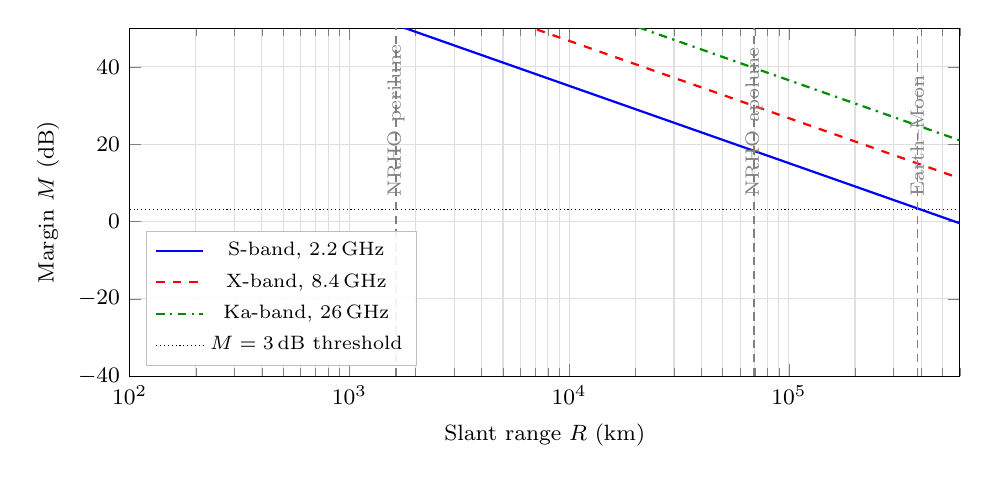
\begin{tikzpicture}
\begin{axis}[
    width=\columnwidth, height=6cm,
    xlabel={Slant range $R$ (km)},
    ylabel={Margin $M$ (dB)},
    xmode=log, xmin=100, xmax=600000,
    ymin=-40, ymax=50,
    grid=both, grid style={gray!25},
    tick label style={font=\footnotesize},
    label style={font=\footnotesize},
    legend style={font=\scriptsize, at={(0.02,0.03)}, anchor=south west,
                  draw=gray!50, fill=white, fill opacity=0.9,
                  text opacity=1, row sep=1pt},
]
\addplot[blue, thick, domain=100:600000, samples=120]
  {10*log10(40)+10*log10(0.6*(pi*0.75*2.2e9/2.998e8)^2)+10*log10(0.6*(pi*34*2.2e9/2.998e8)^2)-20*log10(4*pi*x*1e3*2.2e9/2.998e8)+228.6-10*log10(44)-2-10-10*log10(1e8)};
\addlegendentry{S-band, 2.2\,GHz}
\addplot[red, thick, dashed, domain=100:600000, samples=120]
  {10*log10(40)+10*log10(0.6*(pi*0.75*8.4e9/2.998e8)^2)+10*log10(0.6*(pi*34*8.4e9/2.998e8)^2)-20*log10(4*pi*x*1e3*8.4e9/2.998e8)+228.6-10*log10(44)-2-10-10*log10(1e8)};
\addlegendentry{X-band, 8.4\,GHz}
\addplot[green!55!black, thick, dashdotted, domain=100:600000, samples=120]
  {10*log10(40)+10*log10(0.6*(pi*0.75*26e9/2.998e8)^2)+10*log10(0.6*(pi*34*26e9/2.998e8)^2)-20*log10(4*pi*x*1e3*26e9/2.998e8)+228.6-10*log10(44)-2-10-10*log10(1e8)};
\addlegendentry{Ka-band, 26\,GHz}
\addplot[black, densely dotted, domain=100:600000] {3};
\addlegendentry{$M=3$\,dB threshold}
\draw[gray, densely dashed] (axis cs:1629,-40) -- (axis cs:1629,50);
\node[gray, font=\scriptsize, rotate=90, anchor=west, inner sep=2pt]
  at (axis cs:1629,5) {NRHO perilune};
\draw[gray, densely dashed] (axis cs:69363,-40) -- (axis cs:69363,50);
\node[gray, font=\scriptsize, rotate=90, anchor=west, inner sep=2pt]
  at (axis cs:69363,5) {NRHO apolune};
\draw[gray, densely dashed] (axis cs:384000,-40) -- (axis cs:384000,50);
\node[gray, font=\scriptsize, rotate=90, anchor=west, inner sep=2pt]
  at (axis cs:384000,5) {Earth--Moon};
\end{axis}
\end{tikzpicture}
\caption{Delivered margin against slant range at three carrier frequencies, with $D_t=\SI{0.75}{m}$, $D_r=\SI{34}{m}$, $P_t=\SI{40}{W}$, $T_{\mathrm{sys}}=\SI{44}{K}$ and $R_b=\SI{100}{Mbps}$. Both antenna gains are frequency-dependent, so higher frequencies yield a net \SI{6}{dB} per octave advantage.}
\label{fig:margin}
\end{figure}

\subsection{Required Aperture Against Range}
Fig.~\ref{fig:aperture} shows the transmit aperture required to sustain a \SI{3}{dB} margin at Ka-band against a \SI{34}{m} receive aperture, for data rates of 1, 10 and \SI{100}{Mbps}. The required aperture scales linearly with range and as the square root of the data rate, as predicted by \eqref{eq:aperture}. At \SI{384000}{km} and \SI{100}{Mbps} the curve returns $D_t \approx \SI{0.06}{m}$ for the \SI{3}{dB} threshold, far smaller than the \SI{0.75}{m} used in the worked example; the difference reflects the \SI{22}{dB} by which the worked example exceeds the \SI{3}{dB} closure threshold. At a range of \SI{1629}{km}, the perilune altitude of an NRHO (which lies over the north pole, so that a south-polar user sees the relay near apolune), the requirement falls to sub-millimetre values, which indicates that a surface-to-relay link at short range is not aperture-limited when the far end is a large ground antenna. That condition does not hold in practice: when the receiver is a \SI{0.5}{m} relay antenna, the required transmit aperture rises by a factor of approximately sixty-eight ($34/0.5$), which is why link~2 of Table~\ref{tab:links} is classified as aperture-constrained.

\begin{figure}[!t]
\centering
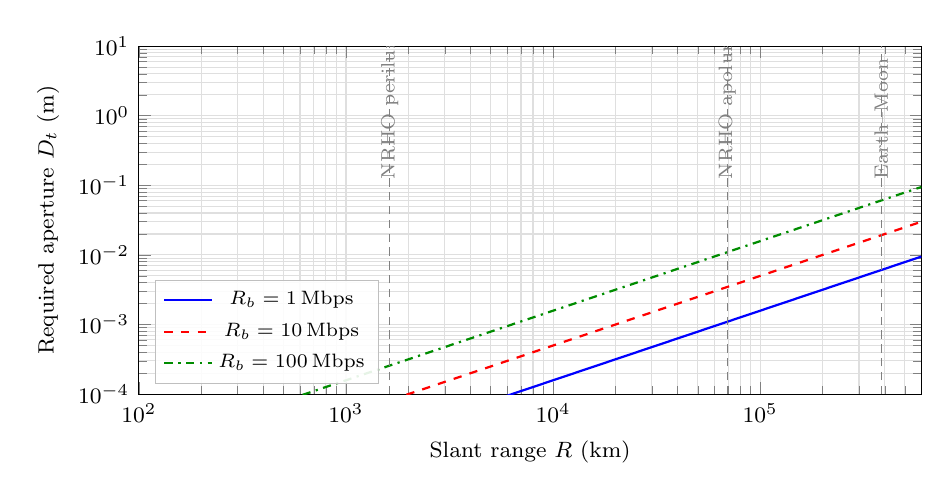
\begin{tikzpicture}
\begin{axis}[
    width=0.95\columnwidth, height=6cm,
    xlabel={Slant range $R$ (km)},
    ylabel={Required aperture $D_t$ (m)},
    ylabel near ticks,
    xmode=log, ymode=log,
    xmin=100, xmax=600000,
    ymin=1e-4, ymax=10,
    grid=both, grid style={gray!25},
    tick label style={font=\footnotesize},
    label style={font=\footnotesize},
    legend style={font=\scriptsize, at={(0.02,0.03)}, anchor=south west,
                  draw=gray!50, fill=white, fill opacity=0.9,
                  text opacity=1, row sep=1pt},
]
\addplot[blue, thick, domain=100:600000, samples=120]
  {4*x*1e3*0.01154/(pi*0.6*34)*sqrt(1.38e-23*44*1e6*1.585*19.95/40)};
\addlegendentry{$R_b=1$\,Mbps}
\addplot[red, thick, dashed, domain=100:600000, samples=120]
  {4*x*1e3*0.01154/(pi*0.6*34)*sqrt(1.38e-23*44*1e7*1.585*19.95/40)};
\addlegendentry{$R_b=10$\,Mbps}
\addplot[green!55!black, thick, dashdotted, domain=100:600000, samples=120]
  {4*x*1e3*0.01154/(pi*0.6*34)*sqrt(1.38e-23*44*1e8*1.585*19.95/40)};
\addlegendentry{$R_b=100$\,Mbps}
\draw[gray, densely dashed] (axis cs:1629,1e-4) -- (axis cs:1629,10);
\node[gray, font=\scriptsize, rotate=90, anchor=west, inner sep=2pt]
  at (axis cs:1629,0.1) {NRHO perilune};
\draw[gray, densely dashed] (axis cs:69363,1e-4) -- (axis cs:69363,10);
\node[gray, font=\scriptsize, rotate=90, anchor=west, inner sep=2pt]
  at (axis cs:69363,0.1) {NRHO apolune};
\draw[gray, densely dashed] (axis cs:384000,1e-4) -- (axis cs:384000,10);
\node[gray, font=\scriptsize, rotate=90, anchor=west, inner sep=2pt]
  at (axis cs:384000,0.1) {Earth--Moon};
\end{axis}
\end{tikzpicture}
\caption{Transmit aperture required for a \SI{3}{dB} margin at Ka-band against slant range, for three data rates, with $D_r=\SI{34}{m}$, $P_t=\SI{40}{W}$, $T_{\mathrm{sys}}=\SI{44}{K}$ and $\eta=0.6$.}
\label{fig:aperture}
\end{figure}

\subsection{Gain and Beamwidth Against Aperture}
Fig.~\ref{fig:gainbw} shows the gain and the half-power beamwidth of a Ka-band aperture as functions of its diameter, on separate vertical scales. A \SI{0.75}{m} antenna provides approximately \SI{44}{dBi} of gain with a beamwidth of approximately \SI{1.1}{\degree}, whereas a \SI{34}{m} DSN antenna provides approximately \SI{77}{dBi} with a beamwidth of approximately \SI{0.024}{\degree}. The DSN attains the latter with ground-based pointing infrastructure that is not available on a spacecraft or lander. Conversely, a \SI{0.1}{m} lander antenna has a beamwidth near \SI{8}{\degree}, which relaxes the pointing requirement but yields only approximately \SI{26}{dBi}. The two curves diverge monotonically, which shows graphically the coupling noted in Section~\ref{sec:fundamentals}: the gain that closes the link is inseparable from the pointing requirement that the platform must then meet.

\begin{figure}[!t]
\centering
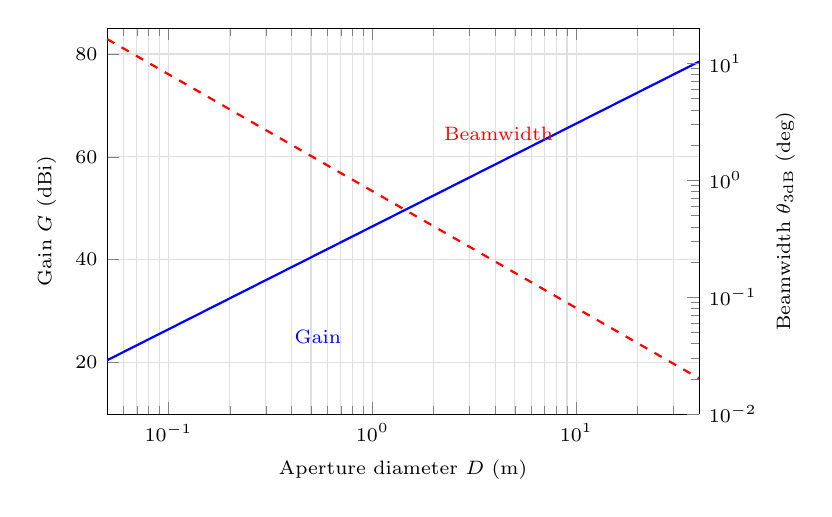
\begin{tikzpicture}
% Left axis: gain. scale only axis keeps both axis bodies identical in size,
% so the two vertical scales align; width is reduced to leave room for both labels.
\begin{axis}[
    name=gainaxis,
    width=0.62\columnwidth, height=4.9cm,
    scale only axis,
    xlabel={Aperture diameter $D$ (m)},
    ylabel={Gain $G$ (dBi)},
    xmode=log, xmin=0.05, xmax=40,
    ymin=10, ymax=85,
    axis y line*=left,
    grid=both, grid style={gray!25},
    tick label style={font=\scriptsize},
    label style={font=\scriptsize},
]
\addplot[blue, thick, domain=0.05:40, samples=90]
  {10*log10(0.6*(pi*x/0.01154)^2)};
\node[blue, font=\scriptsize, anchor=west, inner sep=1pt]
  at (axis cs:0.4,25) {Gain};
\end{axis}
% Right axis: beamwidth on an independent logarithmic scale.
\begin{axis}[
    width=0.62\columnwidth, height=4.9cm,
    scale only axis,
    at=(gainaxis.south west), anchor=south west,
    xmode=log, xmin=0.05, xmax=40,
    ymode=log, ymin=0.01, ymax=20,
    ylabel={Beamwidth $\theta_{3\mathrm{dB}}$ (deg)},
    axis y line*=right,
    axis x line=none,
    tick label style={font=\scriptsize},
    label style={font=\scriptsize},
]
\addplot[red, thick, dashed, domain=0.05:40, samples=90] {70*0.01154/x};
\node[red, font=\scriptsize, anchor=east, inner sep=1pt]
  at (axis cs:8,2.5) {Beamwidth};
\end{axis}
\end{tikzpicture}
\caption{Antenna gain and half-power beamwidth against aperture diameter at \SI{26}{GHz}, plotted on separate vertical scales.}
\label{fig:gainbw}
\end{figure}

\subsection{The Five Canonical Links}
Table~\ref{tab:links} summarizes the five canonical lunar links, numbered as in Fig.~\ref{fig:overview}, each of which is an instance of \eqref{eq:aperture} evaluated at a different slant range. Four of the five are limited by geometry, whether through range, aperture or pointing. The rates of links~2 to~4 assume $P_t = \SI{10}{W}$, a \SI{500}{K} receiver on the relay, $L_{\mathrm{o}} = \SI{2}{dB}$ and uncoded QPSK. Under these assumptions the \SI{0.5}{m} pair of link~2 closes \SI{1}{Mbps} only to about \SI{8000}{km}, and at the \SI{70000}{km} apolune of an NRHO its rate falls to about \SI{14}{kbps}, which is why link~2 is limited by the aperture that a surface terminal can carry. The trunk link to Earth is the exception: it is limited by weather availability and by contention for ground-station time, because the \SI{34}{m} aperture is large enough that the range is no longer the binding term.

\begin{table*}[!t]
\caption{The Five Canonical Lunar Links and Their Dominant Constraints. Values Are Indicative}
\label{tab:links}
\centering
\footnotesize
\begin{tabularx}{\textwidth}{@{}lrlllrR@{}}
\toprule
Link & Range & Band & Aperture, Tx / Rx & Beamwidth & Data rate & Dominant constraint \\
\midrule
1. Surface access & 1--10\,km & S, 2.4\,GHz & omni / omni & --- & 1\,Mbps & Terrain blockage \\
2. Surface-to-relay & 1\,000--70\,000\,km & S, 2.2\,GHz & 0.5 / 0.5\,m & 19\textdegree & 1\,Mbps to 14\,kbps & Surface aperture \\
3. Surface-gateway backhaul & 8\,700--70\,000\,km & Ka, 26\,GHz & 1.5 / 1.5\,m & 0.5\textdegree & 10--100\,Mbps & Aperture and pointing \\
4. Inter-satellite & 60\,000\,km & Ka, 26\,GHz & 1 / 1\,m & 0.8\textdegree & ${\approx}40$\,Mbps & Aperture and power \\
\phantom{4. }(optical variant) & 60\,000\,km & 1550\,nm & 10 / 10\,cm & 19\,\textmu rad & 1\,Gbps & Pointing accuracy \\
5. Trunk to Earth & 384\,000\,km & Ka, 26\,GHz & 0.75 / 34\,m & 1.1\textdegree / 0.024\textdegree & 0.1--1\,Gbps & Weather, scheduling \\
\bottomrule
\end{tabularx}
\end{table*}

\subsection{Surface Access Link}
Link~1 in Table~\ref{tab:links} is the surface access link, connecting a rover, lander or suited astronaut to a local relay at \SI{1}{}--\SI{10}{km}. The dominant constraint is terrain blockage rather than path loss. At \SI{2.4}{GHz} with omnidirectional antennas, the free-space loss over \SI{10}{km} is only \SI{120}{dB}. For $T_{\mathrm{sys}} = \SI{290}{K}$, $L_{\mathrm{o}} = \SI{2}{dB}$ and the uncoded requirement of Table~\ref{tab:budget}, a \SI{1}{W} (\SI{0}{dBW}) transmitter with a \SI{3}{dBi} receive antenna closes the link with approximately \SI{15}{dB} of margin at \SI{1}{Mbps}.

The access link most closely resembles a terrestrial small cell in its design approach. The study that preceded the first surface network modeled an LTE network-in-a-box mounted on a lander at a height of \SI{15}{} or \SI{30}{m} with \SI{5}{dBi} antennas, and found that links can be supported up to \SI{10}{km}, with a peak uplink rate of \SI{69.95}{Mbps} for a \SI{20}{MHz} Release-8 carrier with 64QAM~\cite{nokia_lunar_3gpp}. Unlike a terrestrial small cell, the cell boundary follows terrain rather than a contour of constant received power, so the planning tool must be a ray tracer operating on a digital elevation model~\cite{azami_terrain_aware,zhu_channel_ray}. The ITU-R Irregular Lunar Model~\cite{itu_p2170} provides the propagation prediction, but as discussed in Section~\ref{sec:measurement} it has not been validated against in-situ measurement at the relevant frequencies and ranges.

\subsection{Surface-Gateway-to-Relay Backhaul}
Link~3 in Table~\ref{tab:links} is the backhaul from a surface gateway or habitat to an orbital relay. This link operates at Ka-band (\SI{26}{GHz}) with directional antennas on both ends, and the dominant constraint is the product of aperture and pointing accuracy. For a south-polar gateway the relevant range is the relay's apolune, where it dwells over the pole. Take $P_t = \SI{10}{W}$, $T_{\mathrm{sys}} = \SI{500}{K}$ at the relay, $L_{\mathrm{o}} = \SI{2}{dB}$, uncoded QPSK and $R_b = \SI{10}{Mbps}$. A pair of \SI{0.5}{m} antennas then closes with \SI{5.0}{dB} of margin at the \SI{17400}{km} apolune of the LCRNS reference ELFO~\cite{lcrns_ref_const}, whereas the margin falls to \SI{-7.0}{dB} at the \SI{69400}{km} apolune of the NRHO. The \SI{12}{dB} range penalty is recovered either by a sixteen-fold reduction in data rate or by enlarging both antennas to approximately \SI{0.9}{m} for a \SI{3}{dB} margin, since the required aperture product grows with the fourfold range ratio and each diameter with its square root. The backhaul is thus coupled to orbit selection: an NRHO relay demands roughly twice the antenna diameter at both ends compared with an ELFO relay, which narrows the Ka-band beam from \SI{1.6}{\degree} to approximately \SI{0.9}{\degree} and tightens the pointing requirement accordingly.

The relay link also carries the timing reference for the surface network. In the Intuitive Machines LCRNS design, each relay's onboard time is synchronized to GPS time by a GNSS receiver and held between updates by an ultra-stable oscillator~\cite{ansalone_lcrns_time}, and the relays broadcast a navigation signal from which surface users derive time~\cite{dafesh_afs}. The \SI{56.02}{\micro\second\per day} relativistic rate offset between lunar and terrestrial clocks~\cite{ashby_lunar_time} is predictable and is removed by modeling; what a surface node cannot remove is the drift of its own oscillator while no relay is in view, which grows with the instability of the oscillator and the length of the outage (Section~\ref{sec:pnt}).

\subsection{Optical Inter-Satellite Budget}
With \SI{1}{m} dishes at both ends, \SI{10}{W} and a \SI{500}{K} receiver, the radio-frequency inter-satellite link at \SI{60000}{km} supports only about \SI{40}{Mbps} at zero margin. An optical implementation closes with positive margin at comparable aperture sizes. Taking $\lambda = \SI{1550}{nm}$, $P_t = \SI{+5}{dBW}$ (\SI{3}{W}), $D_t = D_r = \SI{10}{cm}$, $\eta = 0.5$, $R_b = \SI{1}{Gbps}$ and differential phase-shift keying with an optically preamplified receiver, the telescope gain is \SI{103.1}{dB} at each terminal and the free-space loss is \SI{293.7}{dB}. For a Gaussian beam the pointing loss is approximately $\exp(-G_t\theta_e^2)$ for a pointing error $\theta_e$, which amounts to \SI{0.8}{dB} at $\theta_e = \SI{3}{\micro\radian}$ against a beamwidth of $1.22\lambda/D = \SI{18.9}{\micro\radian}$. The received power is then $5 + 103.1 + 103.1 - 293.7 - 0.8 = \SI{-83.3}{dBW}$. An uncoded preamplified DPSK receiver requires approximately 25~photons per bit~\cite{caplan_laser_comm}, or \SI{-84.9}{dBW} at \SI{1}{Gbps}, so the margin is \SI{1.6}{dB} before any coding gain.

The pointing allowance dominates the sensitivity of this budget. The best pointing accuracy demonstrated on a lunar optical link is \SI{2.5}{\micro\radian}, achieved by the Lunar Laser Communication Demonstration~\cite{boroson_llcd}. Doubling the pointing error to \SI{5}{\micro\radian} raises the pointing loss to approximately \SI{2.2}{dB}, which consumes almost all of the margin, and because the loss grows with the square of the error the link no longer closes at \SI{6}{\micro\radian}. Flight results supporting these parameters include optical downlinks from lunar and low-Earth-orbit missions demonstrating \SI{200}{}--\SI{260}{Mbps} with apertures of \SI{10}{}--\SI{22}{cm}~\cite{nasa_o2o,tbird_optical}, and proposed Moon-to-Earth links targeting \SI{2.5}{Gbps}~\cite{jaxa_optical_relay}. No inter-satellite optical link at cislunar range has yet been demonstrated in flight; the parameters above are consistent with the ISOC design, which targets gigabit connectivity among lunar smallsats with a multi-telescope omnidirectional terminal~\cite{isoc_2026}.


\section{Environmental Constraints}
\label{sec:environment}

We summarize the lunar environmental parameters that enter link design. The dielectric permittivity of the regolith follows $\varepsilon_r' = (1.93 \pm 0.17)^{\rho}$ for bulk density $\rho$ in \si{g/cm^3}~\cite{olhoeft_strangway1975}, with a loss tangent between $10^{-3}$ in the highlands and $10^{-2}$ in the mare basalts at S-band; measurements on Chang'e-5 samples extend these figures to \SI{0.2}{}--\SI{12.2}{GHz}~\cite{dong_dielectric_ce5}. A surface antenna therefore operates above a ground plane with $\varepsilon_r$ between 2 and 3, which perturbs the radiation pattern but is second-order by comparison with terrain blockage. Median surface slopes range from \SI{3}{}--\SI{5}{\degree} in the maria to \SI{5}{}--\SI{10}{\degree} in the highlands on a \SI{1}{km} baseline~\cite{rosenberg_terrain2011}.

Surface temperatures range from \SI{390}{K} at lunar noon to \SI{95}{K} before sunrise at the equator~\cite{williams_thermal2017}, and the coldest permanently shadowed regions reach approximately \SI{30}{}--\SI{40}{K}~\cite{paige_psr2010}. The surface dose rate is \SI{13.2}{\micro\gray\per\hour}~\cite{zhang_radiation2020}, corresponding to an annual galactic cosmic-ray dose of \SI{416}{mSv}~\cite{naito_radiation}. The lunar day is \SI{29.5}{Earth-days} with a night of \SI{14.77}{Earth-days}~\cite{lunar_sourcebook}, so that a solar-powered node must store energy for \SI{354}{hours} of darkness.

Propagation over lunar terrain is addressed by ITU-R Recommendation P.2170-0, which defines the Irregular Lunar Model for point-to-area and point-to-point attenuation~\cite{itu_p2170}. It is the only standardized lunar surface propagation model, although as discussed in Section~\ref{sec:measurement} it has not been validated against in-situ measurement.


\section{Design Guidelines}
\label{sec:guidelines}
This section condenses Sections~\ref{sec:fundamentals} to~\ref{sec:environment} into rules for first-order sizing. Table~\ref{tab:scaling} collects the scaling relations, and Fig.~\ref{fig:flow} orders the design decisions from the choice of relay orbit to the verification of pointing.


\subsection{Scaling Laws}
Table~\ref{tab:scaling} collects the scaling relations that follow from \eqref{eq:gain} and \eqref{eq:aperture}. They permit a first-order aperture estimate to be formed from the orbit, the data rate and the carrier frequency alone, without evaluating the full budget.

\begin{table}[!t]
\caption{Scaling Relations for First-Order Aperture Sizing}
\label{tab:scaling}
\centering
\footnotesize
\begin{tabularx}{\columnwidth}{@{}lR@{}}
\toprule
Relation & Consequence for design \\
\midrule
$D_t D_r \propto R$ & Doubling the range doubles the aperture product \\
$D_t D_r \propto \sqrt{R_b}$ & Quadrupling the rate doubles the aperture product \\
$D_t D_r \propto \lambda$ & Higher frequency reduces aperture, narrows beam \\
$G \propto (D/\lambda)^2$ & Doubling $D$ adds \SI{6}{dB} and halves the beamwidth \\
Both apertures fixed & Frequency wins: net \SI{6}{dB} per octave \\
Both gains fixed & Path loss wins: net \SI{-6}{dB} per octave \\
One aperture, one gain fixed & Cancellation: margin unchanged \\
Margin criterion & Mean margin $\geq 2\sigma$ (telemetry), $3\sigma$ (command) \\
\bottomrule
\end{tabularx}
\end{table}

\subsection{Decision-Flow Procedure}
Fig.~\ref{fig:flow} sets out the order in which the parameters of \eqref{eq:aperture} are fixed in practice. The orbit is selected first, since it is the parameter over which the communications engineer has least control and which determines the range. The data rate and modulation follow, then the carrier frequency and the available transmit power. Whether one aperture is fixed determines whether \eqref{eq:aperture} is solved for a single unknown or under the additional constraint of a symmetric pair. The margin test then either terminates the procedure or returns it to the aperture, the data rate, or the decision to operate in store-and-forward mode.

\begin{figure}[!t]
\centering
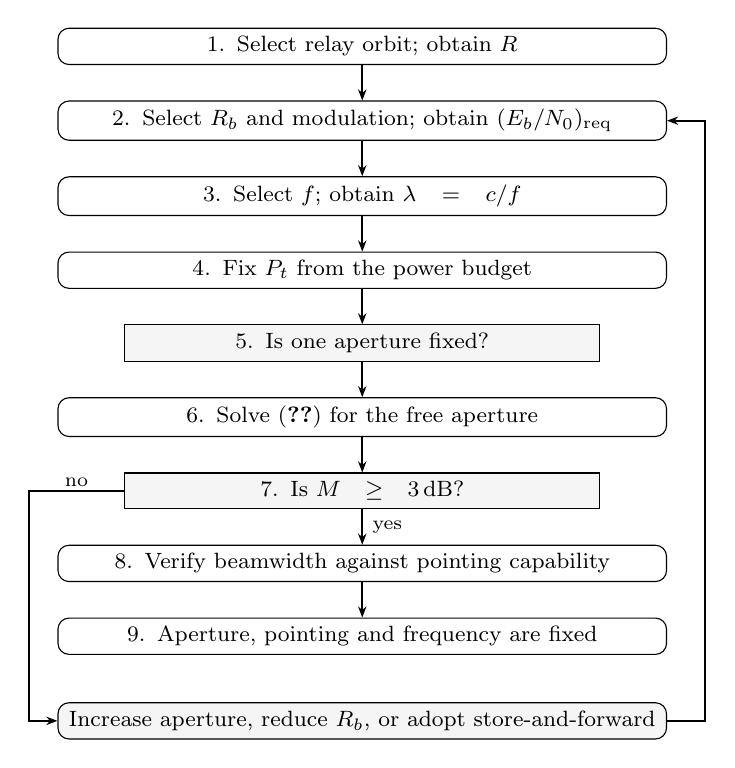
\begin{tikzpicture}[
    node distance=4.5mm,
    box/.style={draw, rounded corners, align=center,
                text width=0.62\columnwidth, inner sep=3pt, font=\footnotesize},
    dec/.style={draw, align=center, text width=0.48\columnwidth,
                inner sep=3pt, font=\footnotesize, fill=gray!8},
    ar/.style={-{Stealth[length=4pt]}, thick},
]
\node[box] (a) {1. Select relay orbit; obtain $R$};
\node[box, below=of a] (b) {2. Select $R_b$ and modulation; obtain $(E_b/N_0)_{\mathrm{req}}$};
\node[box, below=of b] (c) {3. Select $f$; obtain $\lambda=c/f$};
\node[box, below=of c] (d) {4. Fix $P_t$ from the power budget};
\node[dec, below=of d] (e) {5. Is one aperture fixed?};
\node[box, below=of e] (f) {6. Solve \eqref{eq:aperture} for the free aperture};
\node[dec, below=of f] (g) {7. Is $M \geq \SI{3}{dB}$?};
\node[box, below=of g] (h) {8. Verify beamwidth against pointing capability};
\node[box, below=of h] (j) {9. Aperture, pointing and frequency are fixed};
\node[box, below=6mm of j, fill=gray!8] (i) {Increase aperture, reduce $R_b$, or adopt store-and-forward};
\draw[ar] (a)--(b); \draw[ar] (b)--(c); \draw[ar] (c)--(d);
\draw[ar] (d)--(e); \draw[ar] (e)--(f); \draw[ar] (f)--(g);
\draw[ar] (g)--(h) node[midway,right,font=\scriptsize]{yes};
\draw[ar] (h)--(j);
% no: down the left margin to the remedial box
\draw[ar] (g.west) -- ++(-0.10\columnwidth,0)
          node[midway,above,font=\scriptsize,inner sep=1pt]{no} |- (i.west);
% remedial box loops back up the right margin to step 2
\draw[ar] (i.east) -- ++(0.04\columnwidth,0) |- (b.east);
\end{tikzpicture}
\caption{Order in which the parameters of \eqref{eq:aperture} are fixed during lunar link sizing.}
\label{fig:flow}
\end{figure}


\section{Capacity, Mobility and Handover}
\label{sec:capacity}
This section treats the surface segment of Fig.~\ref{fig:overview}. It summarizes the demand against which surface networks are sized, including the robotic users of the current pre-crewed phase, derives the node density set by the radio horizon, and explains why terrain-limited coverage replaces measurement-driven handover with prediction. Table~\ref{tab:demand} lists the user classes with their rate and latency requirements.

\begin{table*}[!t]
\caption{Surface Demand by User Class}
\label{tab:demand}
\centering
\footnotesize
\begin{tabularx}{\textwidth}{@{}>{\raggedright\arraybackslash}p{2.6cm}>{\raggedright\arraybackslash}p{3.6cm}>{\raggedright\arraybackslash}p{4.4cm}>{\raggedright\arraybackslash}X@{}}
\toprule
User class & Traffic & Rate & Binding requirement \\
\midrule
Crewed EVA & Up to four cameras, voice and telemetry & \SI{3}{}--\SI{12}{Mbps} per camera; about \SI{13}{Mbps} uplink for one stream~\cite{nokia_lunar_3gpp} & Continuous coverage of the EVA area \\
Teleoperated rover & Control uplink; video or LiDAR downlink & \SI{384}{kbps} down and \SI{10}{kbps} up (NASA baseline); \SI{1}{Mbps} demonstrated~\cite{lidar_teleops2012} & Control loop closed locally, since the \SI{2.56}{\second} round trip exceeds the reaction time~\cite{ltv_teleops2025} \\
Autonomous multi-robot & Local mesh; bursty return to Earth & Low & Connectivity under terrain shadowing~\cite{cadre_aero2024,banfi_multirover2024} \\
Science & Bulk transfer & \SI{4}{GB/day} for an initial payload; \SI{40}{Mbps} during EVA~\cite{nasa_arts_comm} & Delay-tolerant \\
\bottomrule
\end{tabularx}
\end{table*}


\subsection{Demand Model}
The most detailed public demand model for a lunar surface network is the Nokia Bell Labs study prepared for NASA~\cite{nokia_lunar_3gpp}. It considers up to two astronauts on extravehicular activity with up to four simultaneous cameras at \SI{3}{}--\SI{12}{Mbps} each in 1080p or 4K HEVC, together with voice and telemetry, over a service area of approximately \SI{10}{km}. Against this demand the study evaluates 3GPP peak uplink rates of \SI{69.95}{Mbps} for Release~8 with 64QAM over \SI{20}{MHz}, \SI{149.68}{Mbps} for Release~10 with two-carrier aggregation and 256QAM, and \SI{166}{}--\SI{221}{Mbps} for Release~15 in time-division duplex over \SI{100}{MHz}. The spectrum assumed lies in the lunar surface bands recommended by the SFCG, namely \SI{2.5035}{}--\SI{2.690}{GHz} and \SI{3.500}{}--\SI{3.800}{GHz}, with frequencies below \SI{2}{GHz} excluded in order to protect radio astronomy~\cite{sfcg_rec32}. The study concludes that both LTE and 5G~NR satisfy the mobile-broadband requirement for the planned surface traffic. The demand model remains an unvalidated prediction: the first surface network to fly did not complete a cellular call, and no in-situ traffic data have been published~\cite{nokia_lunar_3gpp}. Subsequent missions carrying updated surface networks and relay satellites are expected to provide the first operational data~\cite{im_ldn_constellation}.

Jia \emph{et al.}~\cite{jia_waveform} recommend OFDMA on the uplink and SC-FDMA on the downlink with \SI{20}{MHz} and \SI{10}{MHz} of bandwidth respectively, \SI{15}{kHz} subcarrier spacing and 4QAM, giving a direct-link range near \SI{6}{km}. That analysis reports peak-to-average power ratio and bit error rate but not aggregate throughput or simultaneous user counts, and should not be read as a capacity result. The BEACON concept~\cite{beacon_demo} proposes a mast of approximately \SI{15}{m} combining power beaming with a 3GPP relay for users within approximately \SI{10}{km}; it describes infrastructure and reports no capacity results.

The demand model above is sized for human extravehicular activity. In the current, pre-crewed phase of lunar exploration, however, all surface users are robotic, and their traffic profile differs from the EVA model. The binding requirement of a teleoperated rover is control-loop latency. The Earth--Moon round trip of \SI{2.56}{\second} exceeds the reaction time of a closed driving loop, so a teleoperation link that crosses the trunk to Earth cannot close a fine control loop: the operator who sees an obstacle in the video feed cannot command a stop before the rover has traveled several meters beyond the frame shown. NASA's Lunar Terrain Vehicle studies confirm this empirically: operators at delays of \SI{0}{} to \SI{8}{\second} all completed a \SI{6}{km} traverse, but average speed fell with latency and workload rose~\cite{ltv_teleops2025}. Fine control must either close locally, within a local surface network that keeps the round trip below human reaction time, or the rover must operate autonomously under supervisory commands that tolerate the trunk delay. In both cases the robot needs continuous coverage of its work area, and the rate requirement is modest: the NASA Human Architecture Team baseline is \SI{384}{kbps} downlink and \SI{10}{kbps} uplink~\cite{lidar_teleops2012}, and a LiDAR-based safeguarded teleoperation system has been demonstrated at \SI{1}{Mbps} with sustained rover speeds of \SI{0.15}{}--\SI{0.25}{m/s}~\cite{lidar_teleops2012}. A recent study derives the data and control channel requirements for LiDAR point-cloud terrain observation over the Moon--Earth link, quantifying the trade-off between sensor resolution, rover speed and the \SI{2.56}{\second} round trip~\cite{lidar_networking2026}. The traffic is asymmetric, continuous during driving windows, and intolerant of interruption.

Autonomous multi-robot exploration adopts the second strategy, which relaxes the latency requirement on the Earth link. The CADRE mission demonstrates three rovers that receive only high-level commands from Earth and then explore, map and perform a multi-static ground-penetrating radar survey autonomously, communicating among themselves through a mesh network and with a base station on the lander~\cite{cadre_aero2024}. The Earth-link traffic is bursty: the rovers collect data during the lunar day and return it when the base station has relay visibility, which is the delay-tolerant model of Section~\ref{sec:protocol}. The inter-rover mesh, by contrast, requires low-latency local exchange of state and map data at low rates and short ranges, which is a surface-to-surface link. Path-planning studies for such swarms show that maintaining connectivity under terrain shadowing is the binding constraint rather than bandwidth~\cite{banfi_multirover2024}, so a rover that enters a shadowed crater is subject to the same loss of coverage as an astronaut.

Science data return from fixed or mobile instruments is the third class, and it is bulk transfer with no latency constraint. The Artemis communication requirements document specifies \SI{4}{GB/day} for an initial science payload mission and \SI{40}{Mbps} downlink during normal EVA~\cite{nasa_arts_comm}. This traffic can use any available contact window and is well matched to the store-and-forward service, but it competes with teleoperation video for the same aperture during crewed periods, which is the contention the scheduling layer of Section~\ref{sec:protocol} must resolve.

\subsection{Node Density}
The Moon has neither atmosphere nor ionosphere, so the radio horizon coincides with the geometric horizon at $d = \sqrt{2 h R_{\mathrm{M}}}$ for mast height $h$ and lunar radius $R_{\mathrm{M}} = \SI{1737}{km}$. A \SI{10}{m} mast therefore reaches \SI{5.9}{km} and a \SI{100}{m} mast reaches \SI{18.6}{km}, in both cases before terrain is taken into account. Node density in a lunar surface network is consequently set by terrain, whereas in terrestrial cell planning it is set by co-channel interference.

\subsection{Mobility in Binary Coverage}
Because coverage is terrain-limited, the received signal is either present at close to full strength or absent altogether. A rover travelling at \SI{1}{}--\SI{5}{m/s} loses the link in under \SI{1}{\second} when the obstructing feature lies within \SI{100}{m}~\cite{azami_terrain_aware}, so the measured signal quality gives no advance warning of the loss. The terrestrial handover trigger, which infers an impending outage from the decay of the serving signal, therefore has no lunar counterpart.

The information is nonetheless available, because the obstruction is static. Lunar topography is mapped and the relay ephemerides are known, so visibility along a planned traverse can be computed in advance; unlike terrestrial fading, which is stochastic, lunar occlusion is deterministic. The trigger consequently moves from measurement to prediction, and three consequences follow. Handover must be initiated while the serving link is still at full strength, which requires a region of overlap with a second visible relay or with a surface relay sited beyond the obstruction, and the extent of that overlap must be sized from the terrain rather than from a fading margin. Where the deployment provides no overlap the rover buffers traffic and forwards it at the next contact, which is the delay-tolerant model~\cite{rfc9171,rfc4838}. Cell planning requires a digital elevation model together with ray tracing~\cite{azami_terrain_aware,zhu_channel_ray}. Where the terrain removes the second link that overlap would require, a passive reflector placed at the obstructing edge can in principle provide one, an idea taken up in Section~\ref{sec:open}.


\section{Constellation Design and Position-Navigation-Timing}
\label{sec:pnt}
This section examines the orbital segment. It compares the orbit families in use or under study, reports published coverage and dilution-of-precision results for the south-polar region, and reviews how position and time are provided without Earth GNSS, from GNSS reception at lunar distance to the definition of a lunar time scale.


\subsection{Orbit Family Comparison}
The choice of relay orbit is the first design decision because it fixes the slant range, which enters the link budget quadratically through the free-space loss and the required aperture product linearly through \eqref{eq:aperture}. Four orbit families are in active use or under study for lunar communications, each trading coverage against range and stationkeeping cost.

\emph{Elliptical Lunar Frozen Orbits} (ELFOs) in the family most often studied have perilune near \SI{900}{km} and apolune near \SI{8700}{km} altitude, inclined approximately \SI{56}{\degree} to the lunar equator~\cite{zhang_elfo_occlusion}; the LCRNS reference design uses a larger ELFO of approximately \SI{1750}{} by \SI{17400}{km} altitude with a period near \SI{30}{hours}~\cite{lcrns_ref_const}. The frozen geometry prevents secular drift of the argument of perilune under the Moon's $J_2$ and mascon perturbations, so stationkeeping is minimal. Because apolune is placed over the south pole, a south-polar user sees the relay during its long dwell at ranges close to the apolune altitude, approximately \SI{8700}{km} and \SI{17400}{km} for the two designs, while the short perilune passage occurs over the northern hemisphere; multiple satellites are needed for continuous coverage. The LCRNS reference design uses five ELFO satellites~\cite{lcrns_ref_const}, and Moonlight plans five satellites in elliptical frozen orbits: one for communications with a \SI{12}{hour} period and a semi-major axis near \SI{6000}{km}, and four for navigation with a \SI{24}{hour} period and a semi-major axis near \SI{10000}{km}~\cite{telespazio_moonlight}.

\emph{Near-Rectilinear Halo Orbits} (NRHOs) are a family of Earth--Moon L2 halo orbits with perilune altitude near \SI{1600}{km} and apolune altitude near \SI{70000}{km}. The long apolune dwell time over the lunar south pole gives near-continuous polar coverage from a single satellite, but its apolune range of approximately \SI{70000}{km} is four to eight times the apolune range of an ELFO, so the aperture product required for the same link is four to eight times larger. NRHO is the orbit selected for the Gateway~\cite{gateway_comm}.

\emph{Low Lunar Orbits} (LLOs) are circular orbits at \SI{100}{}--\SI{200}{km} altitude. They give the shortest slant ranges but are strongly perturbed by mascons. Without stationkeeping, a \SI{100}{km} circular orbit lasts from about two weeks to more than two years depending on inclination~\cite{ramanan_llo}. The Apollo~16 subsatellite, at \SI{11}{\degree} inclination, impacted after 35 days, and only a few frozen inclinations near \SI{27}{\degree}, \SI{50}{\degree}, \SI{76}{\degree} and \SI{86}{\degree} are long-lived~\cite{bell_lunar_orbits}. The $J_2$ nodal regression of the orbit plane is at most about \SI{1.2}{\degree} per day, for an equatorial orbit, and vanishes for a polar one. LLO therefore requires regular stationkeeping; the Lunar Reconnaissance Orbiter flew a \SI{50}{km} circular orbit during its primary mission before moving to a quasi-frozen orbit of approximately \SI{30}{} by \SI{180}{km}~\cite{lro_ka_analysis}.

\emph{Walker constellations} of frozen orbits can provide global navigation, but at a larger scale than the regional designs. Iiyama and Gao~\cite{iiyama_lans} find that at least 99~percent global four-fold coverage requires 16 satellites in a four-plane Walker of circular frozen orbits, and that a PDOP of 6 or better over 99~percent of time and users requires 20 such satellites, or 24 in a Walker of north- and south-elliptical frozen orbits. The \SI{39.2}{\degree} inclination of the circular Walker, measured from the Earth--Moon orbital plane, degrades its high-latitude geometry: for 24 satellites at a semi-major axis of \SI{9751}{km}, the 95th-percentile PDOP rises from 1.8--2.2 within \SI{40}{\degree} of the equator to 3.8--3.9 at \SI{80}{\degree} latitude, and with 10 satellites its south-polar four-fold coverage falls to about 50~percent, against more than 90~percent for a Walker of south-elliptical frozen orbits. Yuan \emph{et al.}~\cite{yuan_hybrid_cislunar} show that a hybrid of Earth--Moon L1/L2 halo, circular lunar and geostationary relay satellites outperforms Walker Star and Walker Delta constellations in age of information at comparable coverage; with six satellites the improvement ranges from 11 to 84~percent depending on the Walker baseline. Trabacchin and Colombatti~\cite{mdpi_orbital_infra} arrive at a different architecture for continuous south-polar service, in which three L2 halo satellites are complemented by one L1 halo satellite.

Table~\ref{tab:orbits} summarizes the trade-off. No single orbit family is optimal for all link types: ELFO minimizes aperture for the surface-to-relay link, NRHO maximizes coverage per satellite, and a Walker constellation provides global navigation at the cost of many more satellites.

\begin{table}[!t]
\caption{Lunar Orbit Families for Relay and Navigation}
\label{tab:orbits}
\centering
\footnotesize
\begin{tabularx}{\columnwidth}{@{}lrrR@{}}
\toprule
Family & Perilune & Apolune & Trade-off \\
\midrule
ELFO & \SI{900}{km} & \SI{8700}{km} & Low range; 5--6~sats for 4-fold (nav) polar visibility \\
NRHO & \SI{1600}{km} & \SI{70000}{km} & 2 halo sats give continuous polar coverage; high aperture \\
LLO & \SI{100}{km} & \SI{200}{km} & Shortest range, orbit unstable \\
Walker (circular frozen) & ${\approx}\SI{8000}{km}$ & ${\approx}\SI{8000}{km}$ & Global nav, ${\geq}16$~sats; polar PDOP about twice equatorial \\
\bottomrule
\end{tabularx}
\end{table}

\subsection{Coverage}
Lunar relay constellations now planned are regional, optimized for the south polar region in which Artemis will operate~\cite{lcrns_ref_const,esa_moonlight_csc}. Published coverage analyses indicate that two large-amplitude halo satellites give continuous single-satellite coverage of one polar region (latitudes above \SI{60}{\degree}) and that four approach complete surface coverage~\cite{gao_halo_coverage}. For an eight-satellite ELFO constellation the probability of four or more satellites being visible is 69~percent, rising to 96~percent for a nine-satellite hybrid of ELFO and NRHO~\cite{zhang_elfo_occlusion}.

Communications availability and navigation availability do not scale together. Communications requires one visible satellite, whereas a navigation fix requires four in favorable geometry: in a six-satellite ELFO model, four or more satellites are visible at the south pole 99~percent of the time, yet the geometric dilution of precision is below 6 only 16~percent of the time~\cite{baweja_dop}.

A global lunar constellation, one that serves all longitudes and latitudes, requires a different architecture from the regional designs above. For radio-frequency links, Cheung and Lee~\cite{cho_relay_coverage} compare a three-orbiter constellation in polar and equatorial orbits with a single relay in an Earth--Moon L2 Lissajous orbit and one in a distant retrograde orbit, and for optical links a multi-hop architecture through an L2 relay and geosynchronous relay satellites. The IOAG lunar communications architecture study~\cite{ioag_lunar_arch} proposes a relay constellation of three to five orbiters in \SI{12}{hour} orbits: frozen elliptical orbits with apolune over the north and south poles and a circular equatorial orbit. The constellation can be built up incrementally, south pole first, then the equator and finally the north pole, and at all latitudes it provides contacts of \SI{5}{}--\SI{7}{hours} with maximum gaps of \SI{1.4}{}--\SI{5.8}{hours}. The distinction between regional and global service is therefore also one of deployment sequence, and the link budget must accommodate the slant range of each stage, which in that design reaches \SI{5892}{km} to the equatorial orbiter and \SI{9672}{km} to an elliptical one.

\subsection{Dilution of Precision}
At the lunar south pole the median geometric dilution of precision (GDOP) is 9.6 for a five-satellite ELFO constellation and 21.5 for a six-satellite one, against a commonly used acceptability threshold of approximately 6; with four satellites a user never sees the four required for a fix~\cite{baweja_dop}. The degradation is geometric in origin: the satellites occupy similar orbital planes and are therefore clustered in the same region of the sky. The GDOP is the square root of the trace of $(H^{\mathsf{T}}H)^{-1}$, where each row of the observation matrix $H$ contains the unit line-of-sight vector to one satellite, augmented by a unit entry for the receiver clock bias. Readers familiar with MIMO communications will recognize $H^{\mathsf{T}}H$ as the analogue of the channel Gram matrix: when the rows of $H$ are nearly parallel, the matrix is ill-conditioned and the position estimate is amplified by the condition number, just as a MIMO channel with correlated columns yields a low multiplexing gain. The lunar south-polar geometry places all visible satellites in a narrow cone, so $H$ is nearly rank-deficient and the condition number is large. Baweja~\cite{baweja_dop} finds that approximately twelve orbital satellites are needed to bring the median below 6, whereas for a user at \SI{-80}{\degree} latitude three surface beacons reduce it from 16.2 to 1.6, matching the performance of a twenty-four-satellite orbital constellation. The surface beacons break the angular degeneracy by adding rows to $H$ with widely differing line-of-sight directions, which is the geometric equivalent of adding well-separated antenna elements to a MIMO array.

\subsection{GNSS at Lunar Distance}
The LuGRE payload on Blue Ghost Mission~1 obtained the first GNSS navigation fix on the lunar surface in March 2025, tracking GPS and Galileo signals at approximately \SI{356000}{km} from Earth~\cite{parker_lugre,nasa_lugre}. Because Earth GNSS is visible only from the near side, far-side users must obtain time and position from the lunar relay constellation. NASA has delivered NavCube3-mini, a GPS and Galileo receiver, for flight on the Altus-1 commercial relay as a technology demonstration of GNSS-based navigation of the relay itself in lunar orbit~\cite{nasa_navcube3_2026}.

\subsection{Lunar Time Scale}
Coordinated Lunar Time is being defined under a United States policy directive~\cite{ostp_ltc}, and the General Assembly of the International Astronomical Union has adopted Resolutions~II and~III establishing the Lunar Celestial Reference System and inviting international agreement on a lunar time standard~\cite{iau_2024_resolutions}. The relativistic rate offset between a clock on the lunar surface and UTC is \SI{56.02}{\micro\second\per day}~\cite{ashby_lunar_time}; the value of \SI{58.7}{\micro\second\per day} quoted in the OSTP memorandum~\cite{ostp_ltc} corresponds to a clock orbiting Earth at the distance of the Moon with the Moon's own gravitational potential neglected, and adding that potential at the lunar surface yields the lower figure~\cite{ashby_lunar_time}. The \SI{56.02}{\micro\second\per day} value is independently corroborated by Kopeikin and Kaplan~\cite{kopeikin_kaplan}, who also identify periodic terms; the monthly term reaches \SI{127}{\micro\second} in barycentric coordinate time but is below \SI{1}{\micro\second} in the comparison between lunar and terrestrial clocks. Two recent papers advance the reference-timescale definition: Bourgoin \emph{et al.}~\cite{bourgoin_ltc} and the unified post-Newtonian framework of Turyshev~\cite{turyshev_2026}, which derives closed-form mappings among TCB, TCG, TT, TCL and TL, with proper-to-coordinate time and two-way time-transfer corrections at sub-picosecond accuracy. In Recommendation CCTF-24-1 (2024), the BIPM Consultative Committee for Time and Frequency confirmed a task group on lunar timing to address the definition and realization of a lunar time scale and its traceability to UTC, and to prepare a draft resolution for the 28th General Conference on Weights and Measures~\cite{bipm_cctf24_1}. Two realizations are under discussion: the coordinate time TCL itself, which Bourgoin \emph{et al.} recommend~\cite{bourgoin_ltc}, or a scaled time matching clocks on a lunar equipotential surface~\cite{ashby_lunar_time}; the latter underlies the LunaNet statement that Coordinated Lunar Time will be referenced to the lunar geoid~\cite{dafesh_afs}. Over a lunar night the offset accumulates to approximately \SI{0.83}{ms}; being predictable, it is removed by modeling. In the Intuitive Machines LCRNS design, each relay's onboard time is synchronized to GPS time by a GNSS receiver and held between updates by an ultra-stable oscillator, with crosslinks and surface receivers used to coordinate the lunar time system~\cite{ansalone_lcrns_time}.


\section{Transfer of 3GPP Non-Terrestrial Concepts}
\label{sec:ntn}

Several architectural elements of 3GPP non-terrestrial networks transfer to the lunar case. The distinction between transparent and regenerative payloads~\cite{3gpp_tr_38821} maps onto the choice between a bent-pipe relay and one performing on-board processing, and the decomposition into feeder and service links~\cite{3gpp_tr_38811,3gpp_ntn_overview} maps onto the lunar trunk and the relay-to-surface link. For beam management, 3GPP reuses the terrestrial NR framework as the NTN baseline, and Release~18 extends NR-NTN to Ka-band terminals in bands n510--n512~\cite{3gpp_tr_38821,3gpp_rp240779}; the same framework is a starting point for lunar relay beams.

These correspondences are analogies; no 3GPP specification applies them to the lunar case. Release~19 introduces regenerative payloads with an on-board gNB, store-and-forward operation with an on-board eNB for IoT-NTN (Work Item~\#1020096), and an NB-IoT NTN TDD mode for the \SI{1.6}{GHz} mobile-satellite band~\cite{3gpp_rel19_ntn}; operation that tolerates a temporary loss of GNSS follows only in Release~20~\cite{3gpp_rp261568}. These additions partially address the lunar delay regime, but no 3GPP work item explicitly targets the lunar or cislunar environment; the scope remains Earth-orbit constellations. The single lunar cellular deployment to date used 4G/LTE in spectrum not allocated for lunar use, under a mission-specific waiver~\cite{mit_tr_nokia}.

Three assumptions embedded in the 3GPP non-terrestrial specifications still fail on the Moon. The first is a maximum slant range of about \SI{41000}{km}, the geostationary case at \SI{10}{\degree} elevation~\cite{3gpp_tr_38821}, against which the lunar trunk of \SI{384000}{km} and \SI{2.56}{\second} round trip places the timer architecture outside its design range. The second is a one-way propagation delay of at most \SI{270.73}{ms}, the transparent geostationary end-to-end value (\SI{541.46}{ms} round trip)~\cite{3gpp_tr_38821}, whereas the lunar surface-to-Earth path is \SI{1.28}{\second} one way. The dashed line in the lower strip of Fig.~\ref{fig:overview} marks this limit: the relay links fall within it and only the trunk to Earth exceeds it. The third is continuous connectivity, whereas lunar relay coverage alternates between contact and outage on a scale of hours; the Release~19 store-and-forward mechanism is specified only for IoT-NTN and covers neither broadband nor real-time service. The assumption that the terminal holds a GNSS fix remains in Release~19, and the Release~20 work only tolerates its temporary loss~\cite{3gpp_rp261568}; on the lunar far side no Earth GNSS is visible at all, and timing advance must be obtained by two-way ranging with the relay or from the lunar navigation service (Section~\ref{sec:pnt}).

Table~\ref{tab:ntn} compares these design values with their lunar counterparts.

\begin{table}[!t]
\caption{3GPP NTN Design Values Against Lunar Values}
\label{tab:ntn}
\centering
\footnotesize
\begin{tabularx}{\columnwidth}{@{}>{\raggedright\arraybackslash}p{2.1cm}>{\raggedright\arraybackslash}p{2.9cm}R@{}}
\toprule
Assumption & 3GPP NTN value & Lunar value \\
\midrule
Slant range & ${\approx}\SI{41000}{km}$ (GEO, \SI{10}{\degree} elevation)~\cite{3gpp_tr_38821} & \SI{384000}{km} on the trunk \\
One-way delay & ${\leq}\SI{270.73}{ms}$ (GEO, transparent)~\cite{3gpp_tr_38821} & \SI{1.28}{\second} \\
Connectivity & Continuous & Contact and outage on a scale of hours \\
Terminal GNSS fix & Assumed in Rel-19; temporary loss in Rel-20~\cite{3gpp_rp261568} & No Earth GNSS on the far side \\
Store-and-forward & IoT-NTN only (Rel-19)~\cite{3gpp_rel19_ntn} & Needed for broadband and bulk data \\
\bottomrule
\end{tabularx}
\end{table}

\subsection{Relay Payload Architecture}
A lunar relay satellite carries three payload classes that determine the spacecraft design. The first is the \emph{bent-pipe transponder}, which receives a signal at one frequency, amplifies it, and retransmits at another, with no on-board processing. Its limitation is that it cannot perform store-and-forward: unless the surface user and the Earth ground station are both in view, the link is idle. A commercial relay designed for store-and-forward is in preparation: SSTL's Lunar Pathfinder, a spacecraft of about \SI{280}{kg} scheduled to launch in 2027, is designed to serve lunar users over S-band and UHF Proximity-1 links and to connect to Earth over a two-way X-band link, holding user data in its payload data recorder until the next Earth contact~\cite{davies_pathfinder_2023,sstl_pathfinder_guide,sstl_pathfinder_mission}. A review of the Chinese Queqiao relay satellites explicitly trades transparent (bent-pipe) against regenerative modes, noting that transparent relays are signal-format-flexible but demand more capable ground stations, while regenerative relays add coding gain under limited on-board resources; Queqiao itself operated in regenerative mode~\cite{queqiao_relay_review_2021}.

The second class is the \emph{regenerative payload}, which demodulates, decodes, and re-encodes the signal on board. 3GPP TR~38.821 defines six reference scenarios, geostationary and low-orbit with transparent and regenerative payloads, and describes regenerative architectures including a functional split in which the gNB distributed unit resides on the satellite and the centralized unit on the ground~\cite{3gpp_tr_38821}. The LunaNet interoperability specification defines both a frame-level real-time relay service that needs no processing of user data and a Bundle Protocol store-and-forward service, which requires a bundle node, and hence demodulation and decoding, at the relay; custody transfer remains an extension still being defined~\cite{lnis_v5}. The LCRNS requirements exclude a bent-pipe design~\cite{nasa_onboard_lunanet}. NASA's onboard processing study for LunaNet data services sizes the on-board processing of a regenerative payload for LCRNS Ka-band data rates of up to \SI{50}{Mbps} with simultaneous S-band, Ka-band and PNT services, and on-board storage for far-side store-and-forward~\cite{nasa_onboard_lunanet}.

The third class is the \emph{navigation payload}, which generates a spread-spectrum navigation signal referenced to an onboard frequency standard. In the Intuitive Machines LCRNS design, each spacecraft's time is steered to GPS time by a GNSS receiver, with an ultra-stable oscillator holding time between fixes~\cite{ansalone_lcrns_time}. The signal is broadcast in the S-band lunar navigation allocation (\SI{2483.5}{}--\SI{2500}{MHz}) of SFCG Recommendation~32-2R7~\cite{sfcg_rec32}. This Augmented Forward Signal, centered at \SI{2492.028}{MHz}, has an in-phase data channel (BPSK(1), \SI{1.023}{Mchip/s}, 500~symbols/s, LDPC-coded) and a dataless quadrature pilot (BPSK(5), \SI{5.115}{Mchip/s}) with the power split equally, and its pilot codes follow the construction of the GPS L1C Weil codes~\cite{lsis_afs,gramling_lunanet_pnt}. Lunar Pathfinder also hosts ESA's NaviMoon GNSS receiver, a \SI{1.4}{kg} payload demonstrating weak-signal GNSS reception from lunar orbit~\cite{esa_navimoon}.

S-band and Ka-band can share one steerable reflector through coaxial or frequency-selective feeds, as on the \SI{0.75}{m} dish of LRO~\cite{lro_ka_analysis}. Relays nevertheless often add a separate wide-beam S-band antenna, because surface access and navigation must cover the whole service area while the Ka-band trunk and backhaul need a narrow, steered beam. On the Gateway, the link to Orion is at S-band through the HALO equipment, and optical terminals are identified only as a future upgrade~\cite{gateway_comm}.


\section{Protocol Design for Intermittent Links}
\label{sec:protocol}

Intermittent connectivity and the Earth--Moon light-time delay jointly govern how protocols must be designed for the lunar environment. The one-way Earth--Moon propagation delay is \SI{1.28}{\second} and the round trip is \SI{2.56}{\second}, which is a lower bound on the duration of any request-response transaction, independent of modulation, coding or protocol. Latency can be reduced only by relocating the responding function closer to the user, whether through on-board processing, edge caching or local authentication.

Wood \emph{et al.} characterize the delay range over which TCP operates through performance and protocol radii fixed by its timers. With the \SI{3}{\second} initial retransmission timeout then in force, the first performance radius corresponds to \SI{1.5}{\second} of one-way delay and the limiting protocol radius, set by SYN retries, to \SI{22.5}{\second}; the authors place direct Earth--Moon TCP inside the first radius, although with poor use of link capacity~\cite{wood_tcp_radius}. RFC~6298 has since lowered the initial timeout to \SI{1}{\second}~\cite{rfc6298}, which moves the first performance radius to \SI{0.5}{\second} of one-way delay and places the Earth--Moon round trip beyond it. Table~\ref{tab:timers} lists the principal timer failures. Delay-tolerant protocols are designed for this regime: the Bundle Protocol Version~7 provides store-carry-forward delivery and, together with its TCP convergence-layer protocol version~4~\cite{rfc9174}, is on the IETF Standards Track~\cite{rfc9171}. Custody transfer, part of the earlier version of the protocol, has been moved out of BPv7 into a separate bundle-in-bundle encapsulation specification~\cite{rfc9171}, and LunaNet lists it as an extension still being defined~\cite{lnis_v5}. The Licklider Transmission Protocol provides reliable delivery over long-delay links~\cite{rfc5326}, and Contact Graph Routing computes routes over scheduled contacts~\cite{burleigh_cgr}. Operational demonstrations in lunar orbit have exercised custody transfer and retransmission under induced outage~\cite{kim_kplo_dtn}. A testbed comparison of end-to-end QUIC against DTN with QUICCL/LTP for the Earth--Moon scenario found that the DTN architecture can outperform end-to-end approaches despite QUIC outperforming TCP~\cite{e2e_vs_dtn_2026}.

\subsection{Vocabularies of the Three Standards Families}
A lunar network is specified by three standards families at once. The space-link and file-transfer layers follow CCSDS, which LunaNet adopts as its interoperability baseline~\cite{lnis_v5,ccsds_lunar_standards}; the surface access layer, where it is proposed, follows 3GPP; and the store-and-forward layer follows the IETF delay-tolerant networking suite, which CCSDS has itself adopted as a companion series~\cite{ccsds_bp,ccsds_ltp}. The three describe overlapping functions in incompatible terms, and an engineer reading across them encounters the same function under three names. Table~\ref{tab:rosetta} maps the functions for which the three families use different mechanisms, omitting those that differ only in name. The recurring pattern is one of scope: a CCSDS mechanism is scoped to a single link, a 3GPP mechanism to an attached subscriber, and a DTN mechanism to a data unit that outlives both.

\begin{table*}[!t]
\caption{Function Names Across the Three Standards Families Governing a Lunar Network}
\label{tab:rosetta}
\centering
\footnotesize
\begin{tabularx}{\textwidth}{@{}>{\raggedright\arraybackslash}p{1.9cm}>{\raggedright\arraybackslash}p{2.9cm}>{\raggedright\arraybackslash}p{2.6cm}>{\raggedright\arraybackslash}p{2.5cm}>{\raggedright\arraybackslash}X@{}}
\toprule
Function & CCSDS / LunaNet & 3GPP & IETF DTN & Substantive difference \\
\midrule
Data unit & Space packet carried in a transfer frame~\cite{ccsds_tm,ccsds_uslp} & Transport block, PDCP PDU & Bundle~\cite{rfc9171} & The bundle carries its own creation timestamp and lifetime in an immutable primary block, so it survives storage and rehoming; frames and PDUs are scoped to one link and are discarded with it \\
Endpoint name & Spacecraft identifier and virtual channel~\cite{ccsds_uslp} & Subscriber and cell identity & Endpoint identifier~\cite{rfc9171} & An endpoint identifier names a service that need not be reachable when addressed, whereas a subscriber identity presumes current attachment and a spacecraft identifier names a vehicle rather than a service \\
Retransmission & COP-1 on the space link~\cite{ccsds_tc}; LTP for long delay~\cite{ccsds_ltp} & HARQ and RLC ARQ & LTP red part~\cite{rfc5326} & HARQ timers are counted in millisecond slots, whereas COP-1 and LTP timers follow the link round trip, about \SI{2.6}{s} on the Earth--Moon link and far longer on interplanetary links, so the same word denotes mechanisms whose retransmission budgets differ by three or more orders of magnitude \\
Path selection & Pre-planned by the ground segment & Path selection in the core network & Contact Graph Routing~\cite{burleigh_cgr} & Contact Graph Routing computes a route over contacts scheduled in the future, whereas the other two select among links available at the moment of the decision \\
Resource scheduling & Pass scheduled in advance and delivered to ground~\cite{ccsds_sle} & Per-slot scheduling at the base station & Contact plan~\cite{fraire_contact_plan} & Scheduling granularity spans sub-millisecond slots to contact windows of hours, so admission control and queueing occupy different layers in each family \\
Security scope & Space Data Link Security, per hop~\cite{ccsds_sdls} & Subscriber authentication and bearer protection & BPSec, per bundle~\cite{rfc9172} & BPSec protection travels with the data across forwarding nodes, whereas link and bearer security terminate at the far end of the hop or at the network edge \\
\bottomrule
\end{tabularx}
\end{table*}

\begin{table}[!t]
\caption{Terrestrial Protocol Timers Against Earth--Moon Values}
\label{tab:timers}
\centering
\footnotesize
\begin{tabularx}{\columnwidth}{@{}llR@{}}
\toprule
Timer & Terrestrial value & Consequence for lunar links \\
\midrule
TCP initial RTO & 1\,s~\cite{rfc6298} & Spurious retransmission at \SI{2.56}{s} RTT~\cite{wood_tcp_radius} \\
HARQ round trip & $\sim$1\,ms & Terrestrial timing exceeded on any relay service link; NTN scheduling offsets and per-process HARQ disabling~\cite{3gpp_ts_38300} absorb the relay range but not the \SI{2.56}{s} trunk RTT \\
OCSP validation & $<$1\,s & Live response infeasible; pre-distributed CRLs leave a vulnerability window between updates~\cite{koisser_pki_space} \\
DNS resolution & $<$100\,ms & Requires caching or DTN naming \\
\bottomrule
\end{tabularx}
\end{table}

The boundary between real-time and store-and-forward operation may be characterized by the ratio of contact duration to outage duration. An ESA-supported study of quasi-real-time traffic over the Earth--Moon DTN link evaluates bundle delay against a \SI{2.5}{\second} mark~\cite{ulierte_traffic_prio}. The NASA relay services requirements document allots each relay node less than \SI{1}{\second} (TBR) of processing latency for real-time data, excluding light time, within an estimated end-to-end budget of \SI{5}{\second}~\cite{nasa_lunar_relay_srd}. The LunaNet interoperability specification, however, defines the two service types without fixing a numerical boundary between them~\cite{lnis_v5}.

\subsection{The 5G-to-DTN Protocol Boundary}
A lunar surface network built on 3GPP NR provides real-time cellular service within a relay's footprint, but when the relay sets below the horizon the 3GPP protocol stack ceases to function because its timers, handover procedures and authentication exchanges all assume continuous connectivity. The transition from 3GPP operation to delay-tolerant operation is not handled by either protocol stack natively: the Release~19 store-and-forward mode is specified only for IoT-NTN, with a regenerative eNB on board~\cite{3gpp_rel19_ntn}, and BPv7 does not define how a 3GPP bearer should be encapsulated into a bundle.

The boundary therefore requires a gateway function, and two designs are possible. The first is a \emph{protocol proxy} on the surface gateway that terminates the 3GPP stack, buffers pending traffic, and injects it into the DTN as bundles when the relay reappears. This design preserves the 3GPP user-plane interface for the rover but requires the gateway to maintain 3GPP state across the outage. The second is a \emph{convergence layer} that maps 3GPP bearers directly onto BPv7 bundles without proxying, treating the DTN as a transport substrate for 3GPP traffic. This design avoids holding 3GPP state at the gateway but requires modifications to the 3GPP stack, and no such mapping has been specified by 3GPP or the IETF. Either design can be prototyped on the network emulation testbeds for space DTN surveyed by Bull \emph{et al.}~\cite{perreault_testbed}.

The GEM emulation testbed at NASA Glenn addresses the 3GPP side of the boundary. It runs srsRAN 4G base-station and user-equipment software on software-defined radios through a hardware channel emulator loaded with ray-traced lunar channel models, and has emulated two notional Artemis~III EVA traverses served by an eNB and packet core hosted on the lander, reproducing the expected drops in SNR and throughput during terrain shadowing~\cite{nasa_gem_2026}. The testbed does not yet include a DTN segment, and the latency cost of the 3GPP-to-DTN transition has not been reported.

\subsection{Scheduling and Contact Plans}
Contact Graph Routing~\cite{burleigh_cgr} computes the path through a delay-tolerant network by enumerating the contact opportunities, namely the intervals during which two nodes have mutual visibility and sufficient link margin, as a directed graph. The contact plan, which lists all contacts with their start time, duration, and data rate, is the input to CGR and must be generated before routing decisions can be made.

On the Moon the contact plan is deterministic and predictable, because the orbital mechanics are known to high precision and the link margins are determined by geometry rather than by weather or contention. The plan is nevertheless not static. A solar-powered node that enters lunar night has no contacts; an ELFO relay dwells over the south pole near apolune and is out of view for several hours around each perilune; and a rover behind a ridge has no contact until it moves. The plan therefore varies with the power state of each node, the orbit of each relay and the terrain around each surface node. When resource constraints prevent every feasible contact from entering the plan, Fraire and Finochietto~\cite{fraire_contact_plan} select the contacts through a multi-objective design that assigns links fairly among nodes while minimizing the all-to-all route delay under CGR, and propose heuristics because the exact model becomes intractable for large topologies.

In practice, the contact plan must be recomputed whenever the network topology changes, which on the Moon happens on three timescales: orbital (hours, as relays enter and exit visibility), diurnal (weeks, as nodes enter and exit lunar night), and mission (months, as new assets are deployed). The LCRNS requirements accordingly call for onboard scheduling and autonomous initiation of stored-data transmission, with routing configurations updated according to the planned contacts, which requires the regenerative payload discussed in Section~\ref{sec:ntn}~\cite{nasa_onboard_lunanet}.


\section{Security, Power and Spectrum}
\label{sec:spectrum}
This section treats four constraints that lie outside the link budget but constrain every lunar design: security without a reachable certificate authority, power through the lunar night, the selection of frequency bands, and the protection of radio astronomy in the Shielded Zone of the Moon.


\subsection{Security Under Intermittency}
Terrestrial public-key infrastructure relies on near-instant credential validation, and fresh Online Certificate Status Protocol (OCSP) responses are practical only for assets whose round-trip latency is of the order of milliseconds~\cite{foerster_pki}. A lunar node is at a one-way light time of approximately \SI{1.28}{\second} from an Earth-based authority and may be out of contact with it for hours. OCSP requires direct contact with the issuing certificate authority and is therefore unsuitable in its intended form~\cite{koisser_pki_space}, while prefetched revocation information, such as cached certificate revocation lists, OCSP stapling or short-lived certificates, leaves a window in which a compromised credential retains its authority~\cite{foerster_pki}; on a lunar link that window is at least as long as the contact gap. Public-key infrastructure for space networks must tolerate certificate authorities subject to delay and disruption~\cite{foerster_pki,koisser_pki_space}, and location-based authentication has been proposed as a complementary mechanism for cislunar missions~\cite{jedermann_location_auth}.

Bundle Protocol Security~\cite{rfc9172} defines integrity and confidentiality services at the bundle layer. Key management, and with it certificate revocation, is treated as a separate network-management function outside the specification, and replay protection is delegated to the security context, to bundle-lifetime checks and to application-level uniqueness mechanisms~\cite{rfc9172}. Access control and non-repudiation are not among the services it defines. The first formal cryptographic analysis, by Dowling \emph{et al.}~\cite{dowling_bpsec}, establishes security under the default security context, identifies a weakness in message-loss detection, and proposes a strengthened construction. The BPSec COSE security context, currently an IETF Internet-Draft~\cite{bpsec_cose}, defines a COSE profile focused on asymmetric-key algorithms and a PKIX certificate profile for BPSec interoperation. It evaluates certificate validity against the bundle creation time and does not expect verifiers to have the continuous connectivity that OCSP requires. The draft explicitly excludes the issuance and provisioning of certificates and the distribution of revocation lists, so the delay-tolerant revocation problem identified in~\cite{foerster_pki,koisser_pki_space} remains open.

\subsection{Power as a Topology Variable}
A solar-powered surface node must operate through the \SI{354}{h} lunar night, and the energy storage required for that night dominates the mass of a photovoltaic power system~\cite{colozza_power1991}. For a \SI{20}{W} night load the stored energy is \SI{7.08}{kWh}, which at a battery specific energy of \SI{100}{Wh/kg} and full depth of discharge corresponds to approximately \SI{71}{kg} of cells. At lunar-base scale, a parametric study of more than 200 configurations found hybrid solar-nuclear systems to be the most advantageous in terms of mass~\cite{balat_power2021}. For comparison, the LuSEE-Night instrument carries a \SI{7.16}{kWh} lithium-ion battery of \SI{50}{kg}, within a total instrument mass limit of \SI{128}{kg}, to operate through \SI{328}{h} of lunar night~\cite{aguirre_lusee}. Because the power state of each node determines whether it is active, the network topology varies over the lunar day. Contact Graph Routing accommodates scheduled contacts~\cite{burleigh_cgr}, but the contact plan itself must be derived from the illumination and hence the position and date of each node, which couples the routing problem to the power system. Battery-aware contact plan design, developed for a small-satellite constellation in low Earth orbit, incorporates a model of solar infeed and on-board battery state into contact plan construction to control the risk of battery depletion~\cite{fraire_battery_cp}.

\subsection{Frequency and Band Selection}
The choice of carrier frequency for each lunar link follows from the aperture-range scaling of Section~\ref{sec:fundamentals}. For a fixed aperture product, higher frequency reduces the required diameter but narrows the beamwidth (Section~\ref{sec:fundamentals}). The selection is therefore link-dependent.

S-band (\SI{2.0}{}--\SI{2.7}{GHz}) is the usual band for surface access and navigation. Its \SI{11}{}--\SI{15}{cm} wavelength permits omnidirectional or low-gain antennas on rovers and suited astronauts, and the SFCG recommends the \SI{2.400}{}--\SI{2.480}{GHz} and \SI{2.5035}{}--\SI{2.690}{GHz} bands for lunar surface wireless networks and the \SI{2483.5}{}--\SI{2500}{MHz} band for in-situ lunar navigation~\cite{sfcg_rec32}. The same recommendation also lists UHF bands (restricted to use outside the Shielded Zone), \SI{3.5}{}--\SI{3.8}{GHz}, \SI{5.15}{}--\SI{5.835}{GHz}, \SI{5.855}{}--\SI{5.925}{GHz}, \SI{25.25}{}--\SI{25.5}{GHz} and \SI{27.5}{}--\SI{28.35}{GHz} for surface networks, so that S-band is the preferred but not the sole surface option. S-band offers limited bandwidth: within the SFCG-recommended \SI{2.5035}{}--\SI{2.655}{GHz} band the study of~\cite{nokia_lunar_3gpp} obtains peak uplink rates of \SI{69.95}{Mbps} for a single \SI{20}{MHz} carrier with 64QAM and \SI{149.68}{Mbps} with two-carrier aggregation and 256QAM.

K/Ka-band (\SI{22.55}{}--\SI{23.15}{GHz} Earth-to-space and \SI{25.5}{}--\SI{27.0}{GHz} space-to-Earth) is the usual band for the trunk and backhaul links~\cite{sfcg_rec32,lnis_v5} because the \SI{12}{mm} wavelength permits a \SI{1.5}{m} dish to produce \SI{50}{dBi} gain, which is needed to close the \SI{384000}{km} Earth--Moon path. In exchange, the \SI{0.5}{\degree} beamwidth of a \SI{1.5}{m} Ka antenna requires attitude knowledge and control to \SI{0.1}{\degree}, which is within the capability of a relay satellite but not of a rover. Ka-band also suffers atmospheric attenuation at the Earth ground station, which at \SI{26}{GHz} and 99.9~percent availability reaches approximately \SI{9}{}--\SI{19}{dB} at \SI{20}{\degree} elevation at the DSN complexes (Section~\ref{sec:worked})~\cite{itu_p618,islam_ka_band}.

X-band (\SI{7.19}{}--\SI{8.5}{GHz}) is a compromise between S and Ka, offering \SI{4}{cm} wavelength with moderate pointing requirements. It is used for direct-to-Earth links from landers that lack a steerable Ka dish, and is the band of the relay links between the Chang'e-4 relay satellite Queqiao and the far-side lander and rover, whereas Queqiao returns data to Earth at S-band to avoid co-channel interference with the X-band relay return in \SI{8450}{}--\SI{8500}{MHz}~\cite{chen_ce4_relay}. Resolution~680 (WRC-23) includes \SI{7190}{}--\SI{7235}{MHz} and \SI{8450}{}--\SI{8500}{MHz} among the frequency ranges in which the spectrum needs of space research service systems on the lunar surface and between lunar orbit and the lunar surface are to be studied~\cite{itu_wrc23_res680}.

Optical (\SI{1064}{}--\SI{1550}{nm}) is selected for the inter-satellite link and the high-rate trunk when pointing stability permits. The \SI{1.55}{\micro\m} wavelength provides approximately \SI{104}{dBi} gain from a \SI{10}{cm} aperture, but the diffraction-limited divergence $1.22\lambda/D \approx \SI{19}{\micro\radian}$ is approximately 450 times narrower than the \SI{0.54}{\degree} Ka-band beam, so that the required pointing stability is between two and three orders of magnitude finer. Optical links are unaffected by RF spectrum congestion and lie outside the Shielded Zone provisions of Article~22, because the Radio Regulations apply to radio waves of frequencies below \SI{3000}{GHz} (No.~1.5)~\cite{itu_rr2024}, but cannot penetrate clouds and are therefore restricted to the space-to-space segment or to dry-site ground stations.

\subsection{Spectrum and the Shielded Zone}
Table~\ref{tab:spectrum} lists the principal allocated and SFCG-recommended bands. The Shielded Zone of the Moon comprises the area of the lunar surface lying more than \SI{23.2}{\degree} beyond the mean limb as seen from the center of the Earth, together with an adjacent volume of space, both shielded from emissions originating within \SI{100000}{km} of the center of the Earth~\cite{itu_rr2024,itu_ra479}. Within it, No.~22.22 of the Radio Regulations prohibits emissions causing harmful interference to radio astronomy and other passive services in the entire frequency spectrum. Two groups of bands are exempted: those allocated to the space research service using active sensors (No.~22.23), and the space operation, active Earth exploration-satellite and spaceborne radiolocation bands required to support space research, together with radiocommunications and space research transmissions within the zone (No.~22.24). In the exempted bands, where emissions are not prohibited, radio astronomy observations and passive space research in the zone may be protected from harmful interference by agreement between the administrations concerned (No.~22.25)~\cite{itu_rr2024}. The regulatory relationship is thereby inverted with respect to terrestrial practice: on Earth the communications operator is generally the protected party, whereas in the Shielded Zone the passive services are protected and active emitters are confined to the exempted bands. Recommendation ITU-R RA.479-5 further advises that transmitters located in or illuminating the zone avoid the bands of greatest astronomical importance, retain frequency flexibility and coordinate with the radio astronomy service. It also reproduces IAU Resolution~B16, which recommends that Shielded Zone radiocommunications be limited to \SI{2}{}--\SI{3}{GHz}, with an alternative band at least \SI{1}{GHz} wide used on a time-coordinated basis~\cite{itu_ra479}. In line with these provisions, the SFCG restricts its UHF lunar bands to use outside the Shielded Zone~\cite{sfcg_rec32}, and the United States and the SFCG favor S-band over L-band for lunar navigation in order to protect radio astronomy in the zone~\cite{csis_lunar_spectrum}. Preparatory studies for WRC-27 Agenda Item~1.15 are under way in ITU-R Working Party~7B, which is developing draft CPM text and a preliminary draft new Report on sharing studies of space research systems for lunar operations~\cite{wrc27_ai115}. The frequency ranges under study are those listed in Resolution~680 (WRC-23): \SI{390}{}--\SI{406.1}{MHz}, \SI{420}{}--\SI{430}{MHz} and \SI{440}{}--\SI{450}{MHz} (outside the Shielded Zone only), \SI{2400}{}--\SI{2690}{MHz}, \SI{3500}{}--\SI{3800}{MHz}, \SI{5150}{}--\SI{5725}{MHz}, \SI{5775}{}--\SI{5925}{MHz}, \SI{7190}{}--\SI{7235}{MHz}, \SI{8450}{}--\SI{8500}{MHz} and \SI{25.25}{}--\SI{28.35}{GHz}, for possible new or modified space research service allocations~\cite{itu_wrc23_res680}. ITU-R Working Party~7D is concurrently developing threshold levels of interference to radio astronomy in the Shielded Zone~\cite{itu_szm_thresholds}, which will quantify the protection criteria that far-side emitters must meet.

\begin{table}[!t]
\caption{Principal Lunar Spectrum Allocations}
\label{tab:spectrum}
\centering
\footnotesize
\begin{tabularx}{\columnwidth}{@{}llR@{}}
\toprule
Band & Frequency & Use \\
\midrule
S & 2025--2110 / 2200--2290\,MHz & Relay proximity; direct-to-Earth for existing missions~\cite{itu_space_research_handbook,sfcg_rec32} \\
S & 2400--2480 / 2503.5--2690\,MHz & Surface wireless network~\cite{sfcg_rec32} \\
S & 2483.5--2500\,MHz & Lunar navigation~\cite{sfcg_rec32} \\
X & 7190--7235 / 8450--8500\,MHz & Direct-to-Earth; Res.~680 study range~\cite{sfcg_rec32,itu_wrc23_res680} \\
K/Ka & 22.55--23.15 / 25.5--27.0\,GHz & Direct-to-Earth~\cite{lnis_v5} \\
K/Ka & 23.15--23.55 / 27.0--27.5\,GHz & Relay proximity, cross-link~\cite{lnis_v5,sfcg_rec32} \\
Optical & 1064 / 1550\,nm & Inter-satellite, trunk; Orion O2O at 1550\,nm (no ITU allocation)~\cite{nasa_o2o} \\
\bottomrule
\end{tabularx}
\end{table}


\section{The Measurement Gap}
\label{sec:measurement}

Recommendation ITU-R P.2170-0 defines the Irregular Lunar Model for point-to-area and point-to-point attenuation over lunar terrain, treating the exosphere as free space and accounting for terrain irregularity and regolith permittivity between \SI{20}{MHz} and \SI{37}{GHz}~\cite{itu_p2170}; NTIA/ITS maintains a public example implementation~\cite{ntia_ilm_github}. It is the only standardized lunar surface propagation model. A preliminary draft revision is already under development in ITU-R Working Party~3J~\cite{itu_p2170_revision}. A series of JPL studies on south-polar propagation, collected by the Lunar Surface Propagation project of NASA Glenn Research Center~\cite{nasa_grc_lsp_2026}, covers the fading channel on downlinks from the lunar south pole to the DSN~\cite{margot_southpole_fading}, multipath measurements from opportunistic LRO-to-DSN observations~\cite{sanchez_net_multipath_2020}, and a coherent-reflection model for direct-with-Earth links validated against Chandrayaan-3 and IM-1 data~\cite{sanchez_net_coherent_2025}. A hardware-in-the-loop emulation testbed (GEM) has been demonstrated with 4G LTE equipment over lunar surface channel models derived from ray tracing, emulating two notional Artemis~III traverses; Wi-Fi components are planned as a later addition~\cite{nasa_gem_2026}. A site-specific path-loss model at \SI{5.855}{GHz} for Shoemaker Rim~F at the lunar south pole, derived from 3D ray tracing over a high-resolution digital elevation map, reports path-loss exponents of 2.54 for dipole-dipole and 4.33 for omni-dipole configurations, indicating a strong sensitivity to the transmitter antenna pattern that link-budget planning must account for~\cite{shoemaker_rim_2026}.

The model is nonetheless a prediction. It adapts the Longley--Rice irregular-terrain formulation to lunar geometry and takes its terrain from LOLA elevation data and its regolith permittivity from relations derived from Apollo samples~\cite{itu_p2170,ntia_ilm_github,olhoeft_strangway1975}; Chang'e-5 measurements at 0.2--12.2~GHz have since revised those relations~\cite{dong_dielectric_ce5}. It has not been validated against in-situ propagation data. The only calibrated surface-to-surface measurements, from the Apollo~17 Surface Electrical Properties experiment, were made at 1--32~MHz over ranges up to \SI{1.6}{km}~\cite{grimm_sep2018}. Empirical data that do exist comprise the LRO K-band (\SI{26}{GHz}) record of more than eleven million received-signal-strength observations on the orbiter-to-ground link~\cite{lro_ka_analysis}, the Chandrayaan-3 and IM-1 direct-to-Earth multipath observations~\cite{sanchez_net_coherent_2025}, the LRO-to-DSN multipath measurements~\cite{sanchez_net_multipath_2020}, the ROLSES-1 surface recordings of terrestrial shortwave transmissions~\cite{hibbard_rolses2025}, the LLCD and LOCL optical results~\cite{boroson_llcd,giggenbach_locl}, the DRATS terrestrial analogue campaign~\cite{nasa_drats2022}, the KPLO delay-tolerant networking test~\cite{kim_kplo_dtn} and the Chang'e-5 dielectric measurements~\cite{dong_dielectric_ce5}. No calibrated measurements exist of surface-to-surface propagation at VHF or higher frequencies, of surface-to-relay fading at low elevation over lunar terrain, of the channel within permanently shadowed regions, or of the interference environment at the surface from Earth-based emitters above the HF band.

A first campaign adequate to close this gap would require at least two surface nodes, one fixed and one mobile, logging calibrated signal strength at S-band and Ka-band across mare, highland, crater-rim and shadowed-region terrain over a complete day-night cycle. Such a data set would either validate or refute the Irregular Lunar Model and would supply the basis for improved channel models~\cite{itu_p2170,zhu_channel_ray}.


\section{Future Research Directions}
\label{sec:open}
This section collects the open problems identified in Sections~\ref{sec:capacity} to~\ref{sec:measurement}. Each subsection states the problem, the related prior work and what remains open, and Table~\ref{tab:open} lists each direction with the section that motivates it and a concrete deliverable that would close it.

\begin{table*}[!t]
\caption{Open Research Problems and the Deliverables That Would Close Them}
\label{tab:open}
\centering
\footnotesize
\begin{tabularx}{\textwidth}{@{}>{\raggedright\arraybackslash}p{4.2cm}>{\raggedright\arraybackslash}p{2.2cm}>{\raggedright\arraybackslash}X@{}}
\toprule
Direction & Motivated by & Deliverable \\
\midrule
In-situ propagation validation & \S\ref{sec:measurement} & Calibrated S- and Ka-band data set from fixed and mobile nodes over several terrain types and one day-night cycle \\
Proactive handover in binary coverage & \S\ref{sec:capacity} & Visibility predictor combining elevation model, relay ephemeris and rover position that runs within the time to occlusion \\
Passive reflectors & \S\ref{sec:capacity}, \S\ref{sec:spectrum} & Quantitative budget of the reflected leg, including alignment tolerance \\
Reconfigurable surfaces & \S\ref{sec:capacity} & Quantitative analysis of a fixed RIS serving a rover behind a ridge \\
Joint communications-navigation design & \S\ref{sec:pnt} & Joint optimization over orbital satellites and surface beacons \\
Timing advance without GNSS & \S\ref{sec:ntn} & Timing-advance procedure based on two-way ranging or the lunar navigation service \\
Positioning reference signals & \S\ref{sec:pnt} & PRS configuration for the south-polar geometry \\
Delay-tolerant security & \S\ref{sec:spectrum} & Revocation and key management over links that are out of contact for hours; LunaNet security specification \\
Integrated sensing and communications & \S\ref{sec:open} & Surface-sensing waveform and resolution against lunar terrain \\
\bottomrule
\end{tabularx}
\end{table*}


\subsection{In-Situ Propagation Validation}
Section~\ref{sec:measurement} identified the Irregular Lunar Model as the only standardized lunar surface propagation model, but noted that it rests on terrain data and electromagnetic theory and has not been validated in situ. The model supplies predictions for which no validation data exist. Deploying calibrated nodes across several terrain types is logistically demanding; the surface Wi-Fi links and the 3GPP technology demonstration planned for Artemis~III~\cite{nasa_gem_2026} will yield operational data, but no announced mission includes a calibrated propagation campaign across several terrain types. Until such data are obtained, the capacity, coverage and handover results in the literature rest on an unvalidated model, and the associated uncertainty is not quantified.

\subsection{Proactive Handover in Binary Coverage}
The binary-coverage regime of Section~\ref{sec:capacity} removes the measured trigger but leaves the underlying geometry predictable, so handover can in principle be scheduled from a visibility computation rather than detected from a signal. Realizing this requires a predictor that operates on a digital elevation model, is fused with the rover position estimate, and runs within the time available before occlusion. Horizon maps derived from digital elevation models are already used operationally to predict terrain occlusion of scheduled relay and direct-to-Earth passes for the Curiosity rover on Mars~\cite{wiederhold_mars_occlusion}, and elevation-model line-of-sight analysis has been applied to lander--rover communication planning for a lunar mission~\cite{menon_teamindus}. Its accuracy is bounded by two factors that have not been characterized: the resolution of the elevation model relative to the features that actually obstruct the link, since boulders and small-scale relief below the model grid are not represented, and the uncertainty in the rover position estimate, which propagates directly into the predicted occlusion time. The resulting trade-off between premature handover and missed occlusion, and the overlap that a deployment must provide to absorb the residual error, remain open.

\subsection{Passive Reflectors for Shadow-Zone Coverage}
A coverage gap behind a crater rim can be closed geometrically. A passive reflector placed at the obstructing edge, either a flat or shaped metallic panel acting as a passive repeater at radio frequencies or a mirror for optical links, provides a second path from the relay to the shadowed region without adding an active node. A corner-cube retroreflector does not serve this purpose, because it returns the incident wave towards its source. Its advantage on the Moon is twofold: it consumes no power, so it is unaffected by the \SI{14.77}{day} lunar night and does not enter the power-topology problem of Section~\ref{sec:spectrum}, and, having no control state, it adds no node that the routing layer must track. A fixed reflector redirects only waves that arrive within its angular acceptance, so the reflected path exists only while the relay occupies the corresponding region of the sky; for an orbiting relay this availability is a deterministic function of the ephemeris, and for the direct-to-Earth link it is bounded by libration. Its drawbacks lie in the alignment tolerance and in the path-loss budget of the reflected leg, and these have not been quantified for the lunar surface case. The idea is distinct from the reconfigurable intelligent surfaces discussed next: a passive reflector trades orientability for zero power and zero control. Relaying Earth radio signals into a lunar shadowed region by a pair of radio-frequency mirrors on a tower appears in a patent disclosure~\cite{sercel_patent_shadowed}, but no quantitative link analysis of passive reflectors for lunar surface coverage has been published.

\subsection{Reconfigurable Surfaces for Predictable Shadow Zones}
The shadow zones produced by lunar terrain are geometrically predictable, because the Moon has no atmosphere and the topography is static: they are fixed for a surface transmitter, vary only with libration for the direct-to-Earth link, and move deterministically with the ephemeris for an orbiting relay. A surface that reflects or re-radiates the relay signal around an obstruction could therefore extend coverage into a shadowed region without deploying an additional relay. Reconfigurable intelligent surfaces have been proposed for cislunar communications to counteract path loss and directivity constraints~\cite{ris_cislunar2024}, and an RIS on a crater edge has been proposed qualitatively to restore connectivity to a rover exploring the crater~\cite{liyanaarachchi_cislunar}. The analogous Martian configurations, including an RIS at a crater edge serving a user inside the crater, have been analyzed for coverage and localization~\cite{koktas_ris_mars}, but the lunar surface case, in which a fixed RIS redirects a relay signal behind a ridge to a rover in shadow, has not been analyzed quantitatively. The trade-off between the cost of emplacing a passive RIS and that of a second surface relay is an open systems-engineering question.

\subsection{Joint Communications-Navigation Constellation Design}
Most of the constellation designs surveyed in Section~\ref{sec:pnt} optimize communications availability and navigation availability separately. The two objectives conflict: communications favors a small number of satellites in high orbits to maximize dwell time and coverage per satellite, at the cost of a larger aperture (Table~\ref{tab:orbits}), whereas navigation favors a larger number distributed across multiple planes to reduce geometric dilution of precision. Baweja~\cite{baweja_dop} quantifies the navigation side of the trade and shows that a small number of surface ranging beacons augmenting a planned orbital constellation supplies geometric diversity that would otherwise require twelve to twenty-four orbital satellites. Joint designs of orbital constellations that serve both functions have been reported, including a south-polar ELFO constellation in which all satellites provide navigation and a fraction also provide communications, evaluated on positioning accuracy, dilution of precision, data volume and availability~\cite{bhamidipati_constellation_2023}, but the joint optimization across orbital satellites and surface beacons for both services remains open.

\subsection{Timing Advance Without GNSS}
The 3GPP non-terrestrial specifications through Release~19 assume a GNSS fix at the terminal, and the Release~20 work addresses only its temporary loss~\cite{3gpp_rp261568}; a far-side lunar terminal must therefore obtain timing advance by other means, either from two-way ranging with the relay or from a position fix supplied by the lunar navigation service of Section~\ref{sec:pnt}. The signalling required, the accuracy attainable and the interaction with Doppler pre-compensation have not been specified.

\subsection{Positioning Reference Signals for Lunar Localization}
The 5G~NR downlink Positioning Reference Signal, introduced in Release~16, provides a wideband reference whose bandwidth, comb density and periodicity can be configured to trade accuracy against overhead. Gonzalez-Garrido \emph{et al.}~\cite{prs_ntn_plans2023} analyze the delay-estimation accuracy of downlink time-difference-of-arrival positioning when a synchronized constellation of low-Earth-orbit satellites transmits the PRS on a shared carrier, and show that Doppler-induced inter-carrier interference and inter-symbol interference grow with the number of satellites in view, which imposes a trade-off on constellation design. On the lunar far side, where no Earth GNSS is visible, a PRS broadcast from orbital relays or surface beacons could provide the localization that GNSS otherwise supplies. The south-polar geometry, however, clusters the visible satellites in a narrow cone and degrades the dilution of precision~\cite{baweja_dop}, and the adaptation of the PRS configuration to this regime has not been studied.

\subsection{Delay-Tolerant Security}
Terrestrial network security assumes that a device can reach an online authentication server within a round-trip of tens of milliseconds. An online certificate status query, an OAuth token refresh and a TLS handshake all require an interactive exchange with a reachable peer. They become costly when the round trip is measured in seconds and fail when no end-to-end path exists for hours, and RFC~9173 notes that revocation mechanisms relying on a centralized certificate authority can fail in the same way~\cite{rfc9173}. The security architecture must be reversed: credentials travel with the data, since they cannot be fetched on demand, and revocation information must be distributed to nodes before it is needed.

The IETF Bundle Protocol Security specification (BPSec, RFC~9172)~\cite{rfc9172} provides the framework for bundle-layer integrity and confidentiality in a delay-tolerant network. BPSec defines security blocks that are carried within the bundle itself, so that integrity and confidentiality protection persist as the bundle is stored and forwarded across multiple intermediate nodes. The default security contexts in RFC~9173~\cite{rfc9173} specify HMAC-SHA2 for integrity and AES-GCM for confidentiality, both keyed symmetrically, and a COSE security context under development at the IETF profiles COSE and X.509 public-key certificates for BPSec interoperation while placing certificate issuance, provisioning and revocation distribution outside its scope~\cite{bpsec_cose}. Dowling \emph{et al.}~\cite{dowling_bpsec} provide the first formal cryptographic analysis of BPSec under its default security contexts. They prove the protocol secure in a secure-channel model, show that the destination cannot detect the loss of message components, and propose a strengthened construction that provides this detection; they also note that key management is not defined by the relevant RFCs, which defer it to an out-of-band mechanism.

Key management remains unresolved. Koisser \emph{et al.}~\cite{foerster_pki} propose a PKI architecture for space networks whose credential-validation layer tolerates delay and disruption through peer-to-peer epidemic dissemination of compact, verifiable revocation data; in constellation-scale simulation it propagates critical revocation updates orders of magnitude faster than certificate revocation lists or OCSP stapling. The systematization-of-knowledge study by Koisser \emph{et al.}~\cite{koisser_pki_space} surveys PKI and location-privacy challenges in space networks more broadly; it identifies the predictable topology of orbital networks as a property that can be exploited to disseminate revocation information efficiently, and treats location privacy chiefly as the risk that satellites intercepting ground-user transmissions can triangulate the position of the user. Montilla and Montilla~Ochoa~\cite{montilla_dtn_security} present LunaNet-specific security considerations for DTN service providers, noting that BPSec deployment requires tight coordination and administrative trust among the parties involved, and listing shared security contexts and key distribution among the policies that interconnected LunaNet service providers must agree.

Three open problems remain. First, no deployed system performs certificate revocation over a link whose staleness is measured in hours; the epidemic revocation scheme of~\cite{foerster_pki} has so far been evaluated only in simulation. Second, replay protection across long outages requires time-window validation against a shared time reference, but lunar time itself is still being defined (Section~\ref{sec:pnt}), creating a circular dependency between the security and timing architectures. Third, the LunaNet interoperability specification~\cite{lnis_v5} references BPSec but mandates neither BPSec nor any security context: its security section is informational and defers requirements to a separate LunaNet security specification that it lists as to be determined, leaving interoperability at the security layer unresolved. A concrete protocol combining bundle-layer integrity, cached revocation, and time-window replay protection, together with a formal security proof grounded in the lunar timing reference, remains to be developed.

\subsection{Integrated Sensing and Communications}
Integrated Sensing and Communications, an approach in which a single waveform carries both data and radar-like sensing, has been studied for non-terrestrial networks in the 6G context~\cite{isac_ntn2026}. The lunar case is suited to this integration: the relay aperture and power budget are shared between communications and navigation, and the terrain that obstructs the communication link is the same terrain that a rover must detect. A relay that simultaneously provides connectivity and obstacle detection could reduce the sensing payload that a rover must carry. For the orbital segment, Dong and Akan~\cite{dong_cislunarsense} use the Ka-band OFDM relay of the planned Lunar Gateway for monostatic debris detection, deriving the orbit-dependent Cram\'er--Rao bound and an orbit-phase-adaptive allocation of sensing duty cycle against relay throughput. The waveform design, the sensing resolution attainable against surface terrain, and the trade-off between sensing and communications resource allocation have not been characterized for the lunar surface.


\section{Conclusion}
\label{sec:conclusion}

This tutorial has presented a link-budget methodology for lunar communications derived from first principles, together with a survey of the environmental, protocol, and regulatory factors that distinguish the lunar domain from terrestrial practice. The work was motivated by the observation that existing surveys catalog architectures and missions but leave the physical relationship between orbit selection, aperture, and pointing implicit, so that an engineer cannot transfer results from one mission to another without recomputing the link budget. The principal contributions are as follows:

1) We have derived the aperture-range scaling law from the link equation, showing that the required aperture product scales linearly with slant range and wavelength, and as the square root of the data rate. Because the slant range on the Moon is fixed by orbital mechanics, the relay orbit becomes the single design decision from which aperture, pointing, and frequency follow, making system-level trades between orbit, aperture, power, and pointing tractable without repeating the full budget for each candidate architecture.

2) We have surveyed the terrestrial assumptions embedded in standard protocols, security architectures, and spectrum regulations, identifying the numerical thresholds at which they fail on the Moon. The \SI{2.56}{\second} round trip exceeds the timers of TCP, 5G~NR HARQ and 3GPP NTN; the binary coverage regime precludes signal-quality-based handover; the lunar diurnal cycle makes power a topology variable; and the far-side Shielded Zone inverts the regulatory relationship between communications and radio astronomy. Each of these failures has a known mitigation: delay-tolerant protocols, handover predicted from terrain and ephemeris, energy storage or hybrid solar-nuclear power, and operation in the bands that the Radio Regulations exempt within the Shielded Zone, coordinated with radio astronomy.

3) We have provided a decision-flow procedure, a terminology mapping, and a taxonomy of the assumptions that cease to hold, so that an engineer approaching lunar link design can identify the dominant constraint and the design principle that applies. Open research problems have been identified and cross-referenced to the sections that motivate them.

The principal limitation is the absence of in-situ measurement. The propagation model, the capacity estimates, and the handover algorithms rest on prediction that surface campaigns have yet to confirm. The scaling law is less exposed to this limitation, because it rests on free-space propagation, which the airless lunar environment approximates closely wherever the path is unobstructed. The environmental and protocol sections will require revision as operational data become available.

The aperture-range scaling rests only on free-space propagation and therefore applies to other cislunar and interplanetary links once the appropriate slant range is used. At Mars the round trip grows from \SI{2.56}{\second} to approximately \SI{6}{}--\SI{45}{minutes}, and contact gaps extend from hours to days and, near solar conjunction, to weeks. The delay-tolerant architecture surveyed here carries over with longer timers and contact plans, so the methodology extends to Mars surface and orbital links once the range and delay parameters are updated.


\bibliographystyle{IEEEtran}
\bibliography{references}

\end{document}
